\documentclass[12pt,a4paper,oneside]{report}

% =============================================================================
% PACKAGES ET CONFIGURATION GLOBALE
% =============================================================================
\usepackage[utf8]{inputenc}
\usepackage[T1]{fontenc}
\usepackage[english,french]{babel}
\frenchsetup{StandardLists=true}
\usepackage{lmodern}
\usepackage[top=2.5cm, bottom=2.5cm, left=3cm, right=2.5cm, headheight=15pt]{geometry}
\usepackage{setspace}
\onehalfspacing
\usepackage{graphicx}
\graphicspath{{docs/figures/}{figures/}{./}}
\usepackage{xcolor}
\usepackage{amsmath, amssymb}
\usepackage{booktabs}
\usepackage{tabularx}
\usepackage{array}
\usepackage{longtable}
\usepackage{fancyhdr}
\usepackage{titlesec}
\usepackage{enumitem}
\usepackage[most]{tcolorbox}
\usepackage{listings}
\usepackage{microtype}
\usepackage[font=small,labelfont=bf,labelsep=colon]{caption}
\usepackage{float}
\usepackage{url}
\usepackage{parskip}

% =============================================================================
% CHARTE GRAPHIQUE ET COULEURS PROFESSIONNELLES
% =============================================================================
\definecolor{navyBlue}{RGB}{15, 35, 75}
\definecolor{midBlue}{RGB}{25, 70, 140}
\definecolor{steelBlue}{RGB}{50, 100, 170}
\definecolor{accentCyan}{RGB}{0, 150, 190}
\definecolor{lightGray}{RGB}{246, 248, 252}
\definecolor{borderGray}{RGB}{215, 225, 235}
\definecolor{darkText}{RGB}{30, 35, 45}
\definecolor{codeBg}{RGB}{243, 246, 250}
\definecolor{accentOrange}{RGB}{225, 105, 30}
\definecolor{crimsonDark}{RGB}{160, 25, 35}

% Puces de listes
\newcommand{\bpuce}{\textcolor{midBlue}{$\blacktriangleright$}\;}
\newcommand{\subpuce}{\textcolor{steelBlue}{$\bullet$}\;}

% =============================================================================
% HYPERREF
% =============================================================================
\usepackage[
  colorlinks=true,
  linkcolor=navyBlue,
  citecolor=midBlue,
  urlcolor=steelBlue,
  pdftitle={Rapport de Stage de Fin d'Année - AutoCare-AI},
  pdfauthor={FARIDI Marwane},
  pdfsubject={Rapport de Stage PFA - UPF / NewDev}
]{hyperref}

% =============================================================================
% EN-TETES ET PIEDS DE PAGE
% =============================================================================
\pagestyle{fancy}
\fancyhf{}
\fancyhead[L]{\small\slshape\nouppercase{\leftmark}}
\fancyhead[R]{\small\slshape AutoCare-AI --- Stage PFA}
\fancyfoot[C]{\thepage}
\renewcommand{\headrulewidth}{0.4pt}
\renewcommand{\footrulewidth}{0pt}

\fancypagestyle{plain}{%
  \fancyhf{}%
  \fancyfoot[C]{\thepage}%
  \renewcommand{\headrulewidth}{0pt}%
}

% =============================================================================
% STYLE DES TITRES
% =============================================================================
\titleformat{\chapter}[display]
  {\normalfont\bfseries\color{navyBlue}}
  {\flushright\normalsize\scshape\color{midBlue}Chapitre \thechapter}
  {0.5ex}
  {\flushleft\LARGE}
  [\vspace{0.8ex}{\color{navyBlue}\titlerule[1.2pt]}]

\titleformat{name=\chapter,numberless}[block]
  {\normalfont\bfseries\color{navyBlue}\LARGE}
  {}
  {0pt}
  {}
  [\vspace{0.8ex}{\color{navyBlue}\titlerule[1.2pt]}]

\titlespacing*{\chapter}{0pt}{-10pt}{20pt}
\titlespacing*{name=\chapter,numberless}{0pt}{-10pt}{16pt}
\titlespacing*{\section}{0pt}{14pt}{6pt}
\titlespacing*{\subsection}{0pt}{10pt}{4pt}
\titlespacing*{\subsubsection}{0pt}{8pt}{3pt}

% =============================================================================
% BOITES TCOLORBOX PERSONNALISEES
% =============================================================================
\newtcolorbox{problemBox}[1][]{
  colback=white,
  colframe=crimsonDark,
  fonttitle=\bfseries\color{white},
  coltitle=white,
  title={\textbf{Probl\'ematique M\'etier : #1}},
  arc=2.5mm,
  boxrule=1pt,
  left=10pt, right=10pt, top=8pt, bottom=8pt
}

\newtcolorbox{techDecision}[1][]{
  colback=lightGray,
  colframe=midBlue,
  fonttitle=\bfseries\color{white},
  coltitle=white,
  title={\textbf{D\'ecision d'Architecture : #1}},
  arc=2.5mm,
  boxrule=1pt,
  left=10pt, right=10pt, top=8pt, bottom=8pt
}

% Commande d'insertion de figure securisee
\newcommand{\inserfig}[4][0.85\textwidth]{%
  \begin{figure}[H]
    \centering
    \IfFileExists{#2}{%
      \includegraphics[width=#1]{#2}%
    }{%
      \begin{tcolorbox}[colback=lightGray,colframe=borderGray,width=#1,halign=center]
        \textbf{[Figure : #3]}\\[0.15cm]
        \footnotesize\textit{Fichier associ\'e : \texttt{#2}}
      \end{tcolorbox}%
    }
    \caption{#3}
    \label{#4}
  \end{figure}%
}

% Commande d'insertion securisee de deux figures mobiles cote a cote
\newcommand{\inserfigpair}[6]{%
  \begin{figure}[H]
    \centering
    \begin{minipage}[t]{0.48\textwidth}
      \centering
      \IfFileExists{#1}{%
        \includegraphics[width=0.92\linewidth]{#1}%
      }{%
        \begin{tcolorbox}[colback=lightGray,colframe=borderGray,width=0.92\linewidth,halign=center]
          \textbf{[Figure : #2]}\\[0.15cm]
          \footnotesize\textit{Fichier : \texttt{#1}}
        \end{tcolorbox}%
      }
      \caption{#2}
      \label{#3}
    \end{minipage}\hfill
    \begin{minipage}[t]{0.48\textwidth}
      \centering
      \IfFileExists{#4}{%
        \includegraphics[width=0.92\linewidth]{#4}%
      }{%
        \begin{tcolorbox}[colback=lightGray,colframe=borderGray,width=0.92\linewidth,halign=center]
          \textbf{[Figure : #5]}\\[0.15cm]
          \footnotesize\textit{Fichier : \texttt{#4}}
        \end{tcolorbox}%
      }
      \caption{#5}
      \label{#6}
    \end{minipage}
  \end{figure}%
}

% Configuration Listings pour le code Java et JSON
\lstset{
  backgroundcolor=\color{codeBg},
  basicstyle=\ttfamily\footnotesize\color{darkText},
  keywordstyle=\bfseries\color{midBlue},
  commentstyle=\itshape\color{darkText!60},
  stringstyle=\color{accentOrange},
  breaklines=true,
  breakatwhitespace=true,
  showstringspaces=false,
  numbers=left,
  numberstyle=\tiny\color{darkText!50},
  numbersep=8pt,
  frame=single,
  rulecolor=\color{borderGray},
  tabsize=2,
  xleftmargin=10pt,
  framexleftmargin=10pt
}

% =============================================================================
\begin{document}
% =============================================================================

% =============================================================================
% PAGE DE GARDE OFFICIELLE UPF
% =============================================================================
\begin{titlepage}
\begin{center}

\begin{minipage}{0.45\textwidth}
  \begin{flushleft}
    \IfFileExists{docs/figures/logo_upf.png}{%
      
\includegraphics[height=2cm]{docs/figures/logo_upf.png}%
    }{%
      {\bfseries\large UNIVERSIT\'E PRIV\'EE DE F\`ES}%
    }
  \end{flushleft}
\end{minipage}
\hfill
\begin{minipage}{0.45\textwidth}
  \begin{flushright}
    \IfFileExists{docs/figures/logo_newdev.png}{%
      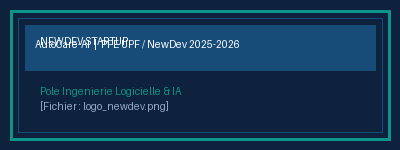
\includegraphics[height=2cm]{docs/figures/logo_newdev.png}%
    }{%
      {\bfseries\large NEWDEV}%
    }
  \end{flushright}
\end{minipage}

\vspace{0.8cm}
{\color{navyBlue}\hrule height 1.2pt}
\vspace{0.3cm}

{\scshape\large Universit\'e Priv\'ee de F\`es --- Facult\'e des Sciences de l'Ing\'enieur}\\
{\small D\'epartement G\'enie Informatique --- 3\textsuperscript{ème} Ann\'ee}

\vspace{1.2cm}

{\LARGE\bfseries\scshape Rapport de Stage de Fin d'Ann\'ee}\\[0.25cm]
{\large\bfseries Projet de Fin d'Ann\'ee (PFA)}\\[0.15cm]
{\small Stage effectu\'e du \textbf{1\textsuperscript{er} f\'evrier 2026} au \textbf{30 juin 2026}}

\vspace{0.9cm}

\begin{tcolorbox}[colback=navyBlue!5, colframe=navyBlue, arc=4pt, boxrule=1.2pt,
    width=0.98\textwidth, halign=center]
  \vspace{0.3cm}
  {\Huge\bfseries\color{navyBlue} AutoCare-AI}\\[0.35cm]
  {\large\bfseries\color{midBlue} Conception et R\'ealisation d'une Plateforme Intelligente\\
  de Maintenance Pr\'edictive et de Jumeau Num\'erique Automobile}\\[0.2cm]
  {\small\itshape\color{darkText} Int\'egrant Mod\'elisation Math\'ematique d'Usure et Diagnostic Assist\'e par IA G\'en\'erative}
  \vspace{0.25cm}
\end{tcolorbox}

\vspace{1.1cm}

\begin{minipage}[t]{0.48\textwidth}
  \begin{flushleft}
    \textbf{Pr\'esent\'e par :}\\[0.2cm]
    {\large\bfseries M. FARIDI Marwane}\\
    {\small \'Elève Ing\'enieur en G\'enie Informatique --- UPF}
  \end{flushleft}
\end{minipage}
\hfill
\begin{minipage}[t]{0.48\textwidth}
  \begin{flushright}
    \textbf{Tuteur de stage :}\\[0.2cm]
    {\bfseries M. Mohamed HAJJOUJI}\\
    {\small CTO / Lead Software Architect}\\
    {\small NewDev, Fès}\\[0.35cm]
    \textbf{Superviseur acad\'emique :}\\[0.2cm]
    {\bfseries Pr. Encadrant P\'edagogique}\\
    {\small D\'epartement G\'enie Informatique, UPF}
  \end{flushright}
\end{minipage}

\vfill

{\small\textbf{Organisme d'accueil :} NewDev --- Fès, Maroc}\\[0.1cm]
{\small\textbf{\'Etablissement d'enseignement :} Universit\'e Priv\'ee de F\`es (UPF)}\\[0.3cm]
{\color{navyBlue}\hrule height 1.2pt}
\vspace{0.3cm}
{\bfseries Ann\'ee Universitaire 2025 -- 2026}

\end{center}
\end{titlepage}

% =============================================================================
% PAGES PRELIMINAIRES
% =============================================================================
\pagenumbering{arabic}
\setcounter{page}{1}

% =============================================================================
% DEDICACES
% =============================================================================
\chapter*{D\'edicaces}
\thispagestyle{plain}

\vspace*{1.8cm}

\begin{center}
\begin{minipage}{0.85\textwidth}
\centering\large\itshape
\`A mes chers parents,\\
qui n'ont m\'enag\'e aucun sacrifice pour m'offrir les meilleures conditions d'\'etude,\\
pour leur affection constante, leurs pri\`eres et leur soutien sans faille\\
tout au long de mon parcours.\\[0.9cm]

\`A ma famille et \`a mes proches,\\
dont la pr\'esence, les encouragements et la bienveillance\\
m'ont port\'e dans les moments les plus exigeants.\\[0.9cm]

\`A mes enseignants de l'Universit\'e Priv\'ee de F\`es,\\
qui ont su me transmettre avec rigueur et passion\\
le go\^ut de l'ing\'enierie logicielle et de l'innovation.\\[0.9cm]

\`A l'\'equipe de NewDev,\\
pour leur accueil chaleureux, leur esprit d'entraide\\
et les pr\'ecieux enseignements partag\'es.\\[1.4cm]

\hfill\textbf{\textsc{FARIDI Marwane}}
\end{minipage}
\end{center}

\clearpage

% =============================================================================
% REMERCIEMENTS
% =============================================================================
\chapter*{Remerciements}
\addcontentsline{toc}{chapter}{Remerciements}

Je tiens tout d'abord \`a exprimer ma profonde gratitude \`a la direction et au corps professoral de l'\textbf{Universit\'e Priv\'ee de F\`es (UPF)}, et plus particuli\`erement au D\'epartement de G\'enie Informatique, pour l'excellence de la formation th\'eorique et pratique dispens\'ee durant mon cursus, ainsi que pour l'opportunit\'e qui m'a \'et\'e offerte d'effectuer ce stage de Projet de Fin d'Ann\'ee (PFA) dans un environnement technologique de premier plan.

Mes remerciements les plus chaleureux s'adressent \`a la soci\'et\'e \textbf{NewDev}, qui a bien voulu m'accueillir au sein de son p\^ole R\&D, m'accordant sa confiance pour mener \`a bien un projet strat\'egique et innovant : la plateforme \textbf{AutoCare-AI}.

Je tiens \`a t\'emoigner ma vive reconnaissance \`a mon tuteur de stage, \textbf{M. Mohamed HAJJOUJI}, CTO et Lead Software Architect chez NewDev. Sa disponibilit\'e permanente, ses conseils avis\'es, sa grande rigueur architecturale et ses retours constructifs ont \'et\'e des moteurs essentiels \`a la r\'eussite de mes missions. Il m'a initi\'e aux meilleures pratiques de l'industrie logicielle contemporaine (Clean Architecture, s\'ecurit\'e d\'efensive, optimisation des performances) et m'a guid\'e avec patience tout au long des diff\'erents sprints.

J'exprime \'egalement ma reconnaissance \`a l'ensemble de l'\'equipe technique de NewDev pour leur accueil convivial, leur esprit de collaboration et les \'echanges fructueux qui ont enrichi mon exp\'erience humaine et professionnelle.

Enfin, je remercie sinc\`erement mon superviseur acad\'emique ainsi que les membres du jury pour le temps qu'ils consacrent \`a l'\'evaluation de ce travail et pour leurs recommandations p\'edagogiques \'eclair\'ees.

\clearpage

% =============================================================================
% RESUME ET ABSTRACT
% =============================================================================
\chapter*{R\'esum\'e}
\addcontentsline{toc}{chapter}{R\'esum\'e}

Le pr\'esent rapport formalise la conception, l'impl\'ementation et l'industrialisation de la plateforme \textbf{AutoCare-AI}, un \'ecosyst\`eme logiciel complet d\'edi\'e \`a la maintenance pr\'edictive automobile et au jumelage num\'erique. Ce projet a \'et\'e r\'ealis\'e dans le cadre d'un stage de Projet de Fin d'Ann\'ee (PFA) de 5 mois au sein de l'entreprise d'ing\'enierie logicielle \textbf{NewDev} \`a F\`es, pour le compte de la 3\textsuperscript{ème} ann\'ee de cursus d'ing\'enieur \`a l'UPF.

Le projet r\'epond \`a un constat r\'ecurrent : la majorit\'e des automobilistes subissent des pannes co\^uteuses et impr\'evues en raison d'une maintenance purement r\'eactive et de l'opacit\'e des diagnostics m\'ecaniques traditionnels. Pour transformer cette dynamique, \textbf{AutoCare-AI} d\'eploie une solution full-stack int\'egr\'ee comprenant :
\begin{itemize}[label=\bpuce]
  \item Un backend robuste sous \textbf{Spring Boot 3 / Java 21} reposant sur une Clean Architecture, assurant la gestion transactionnelle des v\'ehicules, des d\'epenses et des rappels sous PostgreSQL ;
  \item Un moteur de \textbf{Jumeau Num\'erique (Digital Twin)} \'evaluant dynamiquement l'usure de six organes critiques (freinage, suspension, lubrification, pneumatiques, batterie, transmission) via un mod\`ele math\'ematique pond\'er\'e croisant kilom\'etrage et d\'egradation temporelle ;
  \item Un module de \textbf{diagnostic intelligent} exploitant l'API \textbf{Google Gemini Flash}, capable d'interpr\'eter les codes d'anomalies OBD-II et de restituer des explications p\'edagogiques et d\'eterministes en JSON strict ;
  \item Une application mobile fluide d\'evelopp\'ee sous \textbf{React Native / Expo}, adoptant une esth\'etique moderne inspir\'ee des cockpits haut de gamme ;
  \item Une console web d'administration sous \textbf{React} et une cha\^ine \textbf{DevOps} compl\`ete (Docker multi-stage, Docker Compose, pipeline CI/CD GitHub Actions).
\end{itemize}

Le projet totalise 24 endpoints REST s\'ecuris\'es par JWT, 12 \'ecrans mobiles op\'erationnels et une suite de tests unitaires et d'int\'egration validant le syst\`eme avec \textbf{83,7\%} de couverture JaCoCo.

\medskip
\noindent\textbf{Mots-cl\'es :} Jumeau Num\'erique, Maintenance Pr\'edictive, Intelligence Artificielle G\'en\'erative, Google Gemini, Spring Boot 3, React Native, OBD-II, Docker, CI/CD, Clean Architecture.

\clearpage

\chapter*{Abstract}
\addcontentsline{toc}{chapter}{Abstract}

\begin{otherlanguage*}{english}
This report details the requirements analysis, design, implementation, and industrialization of \textbf{AutoCare-AI}, a full-stack automotive predictive maintenance and digital twin platform. This work was conducted during a five-month Final Year Project (PFA) internship at \textbf{NewDev}, a software engineering company based in Fès, Morocco, fulfilling the requirements of the third year of the engineering curriculum at the Private University of Fès (UPF).

The project addresses a critical industry pain point: vehicle maintenance remains overwhelmingly reactive, resulting in unexpected catastrophic component breakdowns, volatile repair expenditures, and information asymmetry between motorists and repair workshops. To overcome these challenges, \textbf{AutoCare-AI} introduces an integrated cyber-physical management platform comprising:
\begin{itemize}[label=\bpuce]
  \item A high-throughput backend built on \textbf{Spring Boot 3 / Java 21} adhering to Clean Architecture principles, handling secure domain transactions and relational persistence on PostgreSQL;
  \item A dedicated \textbf{Digital Twin engine} computing real-time wear coefficients across six critical automotive subsystems (braking, suspension, engine oil, tires, electrical battery, powertrain) based on a dual-parameter mathematical degradation model;
  \item An \textbf{AI-assisted diagnostic engine} leveraging \textbf{Google Gemini Flash}, parsing complex On-Board Diagnostic (OBD-II DTC) failure codes to deliver contextualized, deterministic structured JSON analyses;
  \item A cross-platform mobile application developed with \textbf{React Native / Expo}, offering automotive telemetry monitoring, virtual garage management, and budget planning;
  \item A web-based administration dashboard and an industrial \textbf{DevOps pipeline} (multi-stage Docker builds, Docker Compose service orchestration, GitHub Actions CI/CD workflows).
\end{itemize}

The delivered solution provides 24 secured REST endpoints, 12 functional mobile views, and an automated test suite achieving \textbf{83.7\%} JaCoCo code coverage.
\end{otherlanguage*}

\medskip
\noindent\textbf{Keywords:} Digital Twin, Predictive Maintenance, Generative AI, Google Gemini, Spring Boot 3, React Native, OBD-II, Docker, CI/CD Pipeline, Clean Architecture.

\clearpage

% =============================================================================
% SOMMAIRE ET LISTES
% =============================================================================
\tableofcontents
\clearpage

\listoffigures
\addcontentsline{toc}{chapter}{Liste des figures}
\clearpage

\listoftables
\addcontentsline{toc}{chapter}{Liste des tableaux}
\clearpage

% =============================================================================
% LISTE DES ACRONYMES
% =============================================================================
\chapter*{Liste des Acronymes}
\addcontentsline{toc}{chapter}{Liste des Acronymes}

\begin{table}[H]
\centering
\small
\begin{tabularx}{\textwidth}{p{3.2cm} X}
\toprule
\textbf{Acronyme} & \textbf{D\'efinition Compl\`ete} \\
\midrule
\textbf{API} & Application Programming Interface \\
\textbf{BLE} & Bluetooth Low Energy \\
\textbf{CI/CD} & Continuous Integration / Continuous Deployment \\
\textbf{CORS} & Cross-Origin Resource Sharing \\
\textbf{CRUD} & Create, Read, Update, Delete \\
\textbf{CSRF} & Cross-Site Request Forgery \\
\textbf{DTC} & Diagnostic Trouble Code (Code d'anomalie standard OBD-II) \\
\textbf{DTO} & Data Transfer Object \\
\textbf{ECU} & Electronic Control Unit (Calculateur \'electronique embarqu\'e) \\
\textbf{HTTP / HTTPS} & HyperText Transfer Protocol / Secure \\
\textbf{IDE} & Integrated Development Environment \\
\textbf{JPA} & Java Persistence API \\
\textbf{JSON} & JavaScript Object Notation \\
\textbf{JWT} & JSON Web Token \\
\textbf{LLM} & Large Language Model (Mod\`ele de langage g\'en\'eratif) \\
\textbf{MLD} & Mod\`ele Logique de Donn\'ees \\
\textbf{OBD-II} & On-Board Diagnostics version 2 \\
\textbf{OEM} & Original Equipment Manufacturer (Constructeur automobile) \\
\textbf{ORM} & Object-Relational Mapping \\
\textbf{OWASP} & Open Worldwide Application Security Project \\
\textbf{PFA} & Projet de Fin d'Ann\'ee \\
\textbf{RBAC} & Role-Based Access Control \\
\textbf{REST} & Representational State Transfer \\
\textbf{SaaS} & Software as a Service \\
\textbf{SDK} & Software Development Kit \\
\textbf{SLA} & Service Level Agreement \\
\textbf{SPA} & Single Page Application \\
\textbf{SQL} & Structured Query Language \\
\textbf{UML} & Unified Modeling Language \\
\textbf{UPF} & Universit\'e Priv\'ee de F\`es \\
\textbf{UUID} & Universally Unique Identifier \\
\textbf{VIN} & Vehicle Identification Number (Num\'ero de ch\^assis normalis\'e) \\
\textbf{XSS} & Cross-Site Scripting \\
\bottomrule
\end{tabularx}
\caption*{R\'epertoire des acronymes utilis\'es dans le rapport}
\end{table}

\clearpage

% =============================================================================
% CORPS DU DOCUMENT
% =============================================================================
% =============================================================================
% INTRODUCTION GENERALE
% =============================================================================
\chapter*{Introduction G\'en\'erale}
\addcontentsline{toc}{chapter}{Introduction G\'en\'erale}

\section*{Contexte Global}
L'industrie automobile conna\^it une mutation num\'erique sans pr\'ec\'edent. Jadis consid\'er\'ee comme un simple assemblage m\'ecanique, l'automobile contemporaine est devenue un v\'eritable syst\`eme cyber-physique connect\'e, dot\'e de multiples capteurs, de bus de communication de donn\'ees (CAN bus) et de plusieurs dizaines de calculateurs \'electroniques embarqu\'es (ECU). Chaque trajet g\'en\`ere d\'esormais une multitude d'indicateurs t\'el\'em\'etriques : kilom\'etrage, r\'egime moteur, temp\'eratures, \'etats d'usure et cycles thermiques.

Pourtant, malgr\'e cette richesse de donn\'ees techniques, la gestion de l'entretien automobile par les automobilistes particuliers demeure, encore aujourd'hui, ancr\'ee dans un mod\`ele purement \textbf{curatif et r\'eactif}. L'automobiliste n'intervient que lorsqu'une d\'efaillance majeure se manifeste : apparition d'un voyant d'anomalie critique sur le combin\'e de bord, bruit m\'ecanique anormal ou refus lors de la visite p\'eriodique du contr\^ole technique.

\section*{Probl\'ematique}
Cette gestion r\'eactive g\'en\`ere des cons\'equences \'economiques et s\'ecuritaires n\'egatives manifestes :
\begin{problemBox}[Les Cons\'equences de la Maintenance R\'eactive]
Une n\'egligence mineure (ex. retard sur le renouvellement du liquide de frein ou d\'egradation d'une huile moteur) se propage rapidement aux organes adjacents, provoquant des pannes d\'evastatrices (casse turbo, surchauffe bloc moteur, voilage des disques). Ces incidents imposent des factures impr\'evues atteignant fr\'equemment plusieurs milliers de dirhams et compromettent directement la s\'ecurit\'e routi\`ere des usagers.
\end{problemBox}

Face \`a ce d\'es\'equilibre, la question centrale de ce stage s'articule ainsi :
\begin{center}
\itshape\bfseries\color{navyBlue}
« Comment concevoir et r\'ealiser un \'ecosyst\`eme logiciel int\'egr\'e, ergonomique et s\'ecuris\'e, permettant de transformer chaque v\'ehicule en un Jumeau Num\'erique pr\'edictif et d'exploiter l'Intelligence Artificielle G\'en\'erative pour d\'emocratiser le diagnostic automobile ? »
\end{center}

\section*{Objectifs du Projet}
Pour r\'epondre \`a cette probl\'ematique, le projet \textbf{AutoCare-AI} s'est fix\'e des objectifs techniques et m\'etier ambitieux :
\begin{enumerate}[label=\textbf{\arabic*.}]
  \item \textbf{Mod\'eliser un Jumeau Num\'erique (Digital Twin) :} D\'evelopper un moteur algorithmique capable d'estimer avec pr\'ecision l'indice d'usure r\'eel des diff\'erents organes m\'ecaniques d'un v\'ehicule \`a partir de son kilom\'etrage et de l'anciennet\'e des composants ;
  \item \textbf{Int\'egrer un diagnostic IA d\'eterministe :} Exploiter la puissance du mod\`ele \textbf{Google Gemini Flash} pour traduire des codes de panne OBD-II herm\'etiques en explications claires et recommandations d'action structur\'ees en JSON strict ;
  \item \textbf{Offrir une exp\'erience mobile native :} Concevoir une application \textbf{React Native / Expo} intuitive permettant aux automobilistes de visualiser la sant\'e globale de leur garage, d'enregistrer leurs d\'epenses et de recevoir des alertes pr\'eventives ;
  \item \textbf{Fournir une gouvernance d'entreprise :} D\'evelopper un portail d'administration web sous React pour la supervision des flottes et l'analyse statistique ;
  \item \textbf{Adopter une rigueur d'ing\'enierie logicielle totale :} Couvrir le syst\`eme de tests unitaires et d'int\'egration, s\'ecuriser les \'echanges avec Spring Security 6 / JWT, et industrialiser la solution avec Docker et GitHub Actions.
\end{enumerate}

\section*{D\'emarche d'Ing\'enierie et Outils}
Le projet a suivi une m\'ethodologie Agile/Scrum organis\'ee en six it\'erations (Sprints). La conception a \'et\'e guid\'ee par la mod\'elisation UML (diagrammes de cas d'utilisation, de s\'equence et de classes) et la Clean Architecture. La r\'ealisation s'est appuy\'ee sur IntelliJ IDEA, VS Code, Git, Docker Desktop, Postman et Expo CLI.

\section*{Organisation du M\'emoire}
Le pr\'esent rapport s'organise en \textbf{six chapitres} conformes aux normes acad\'emiques de l'UPF :
\begin{itemize}[label=\bpuce]
  \item \textbf{Chapitre 1 : Contexte G\'en\'eral et Conduite de Projet :} pr\'esente l'entreprise NewDev, l'\'etude concurrentielle et la planification Agile ;
  \item \textbf{Chapitre 2 : Analyse et Sp\'ecification des Besoins :} d\'etaille les acteurs, exigences fonctionnelles/non-fonctionnelles, r\`egles m\'etier, use cases et analyse de risques ;
  \item \textbf{Chapitre 3 : M\'ethodologie et Conception du Syst\`eme :} formalise l'architecture en couches, la mod\'elisation UML, la base de donn\'ees et les choix technologiques ;
  \item \textbf{Chapitre 4 : R\'ealisation de la Plateforme AutoCare-AI :} expose l'impl\'ementation du backend, du Jumeau Num\'erique, du module IA Gemini et de l'app mobile ;
  \item \textbf{Chapitre 5 : Assurance Qualit\'e, S\'ecurit\'e et DevOps CI/CD :} d\'ecrit la strat\'egie de tests, l'audit OWASP, la conteneurisation Docker et le pipeline GitHub Actions ;
  \item \textbf{Chapitre 6 : \'Evaluation, Bilan et Perspectives :} dresse le bilan objectifs vs r\'ealisations, les difficult\'es r\'esolues, les comp\'etences acquises et les axes d'\'evolution.
\end{itemize}

\clearpage
% =============================================================================
% CHAPITRE 1 : CONTEXTE GENERAL ET CONDUITE DE PROJET
% =============================================================================
\chapter{Contexte G\'en\'eral et Conduite de Projet}

\section{Introduction}
Ce premier chapitre pr\'esente l'organisme d'accueil \textbf{NewDev}, analyse la probl\'ematique industrielle du secteur automobile, dresse un benchmark comparatif des solutions existantes et d\'etaille la m\'ethodologie de gestion de projet adopt\'ee.

\section{L'Organisme d'Accueil : NewDev}

\subsection{Identit\'e et Vocation}
\textbf{NewDev} est une soci\'et\'e d'ing\'enierie logicielle fond\'ee \`a F\`es, Maroc, sp\'ecialis\'ee dans la conception de plateformes logicielles innovantes \`a forte valeur ajout\'ee. L'entreprise se distingue par sa culture de la rigueur architecturale, pr\^onant les principes du \textit{Clean Code}, des architectures modulaires et de la s\'ecurit\'e d\`es la conception (\textit{Security by Design}).

\subsection{Domaines d'Expertise}
L'activit\'e de NewDev s'articule autour de quatre domaines strat\'egiques :
\begin{itemize}[label=\bpuce]
  \item \textbf{Ing\'enierie Backend d'Entreprise :} d\'eveloppement d'API REST hautement performantes, architectures microservices sous Java / Spring Boot et Python ;
  \item \textbf{D\'eveloppement Frontend \& Mobile :} applications modernes React, Next.js, et applications mobiles natives et cross-platform sous React Native / Expo ;
  \item \textbf{Solutions d'Intelligence Artificielle :} int\'egration de mod\`eles d'IA g\'en\'erative (LLM), de vision par ordinateur et d'algorithmes d'apprentissage statistique dans les flux d'entreprise ;
  \item \textbf{Pratiques Cloud \& DevOps :} d\'eploiement automatis\'e, orchestration de conteneurs Docker/Kubernetes, et mise en place de pipelines CI/CD.
\end{itemize}

\subsection{Cadre et Environnement du Stage}
Au sein du d\'epartement R\&D de NewDev, j'ai \'et\'e int\'egr\'e comme \'elève ing\'enieur full-stack pour porter le d\'eveloppement complet du projet interne phare : \textbf{AutoCare-AI}. Encadr\'e par \textbf{M. Mohamed HAJJOUJI}, CTO de la structure, j'ai b\'en\'efici\'e d'un suivi m\'ethodologique soutenu, combinant revues de code hebdomadaires, validation des choix d'architecture et transmission des bonnes pratiques industrielles.

\section{Le March\'e et l'Environnement \'Economique}
Quelques indicateurs macro-\'economiques mettent en lumi\`ere l'ampleur du march\'e adress\'e par AutoCare-AI :
\begin{itemize}[label=\bpuce]
  \item Le march\'e mondial de l'apr\`es-vente et de l'entretien automobile (\textit{automotive aftermarket}) est \'evalu\'e \`a plus de \textbf{810 milliards USD} d'ici 2028, enregistrant une croissance annuelle moyenne sup\'erieure \`a 6\,\% ;
  \item Le segment sp\'ecifique de la \textbf{maintenance pr\'edictive automobile} repr\'esente \`a lui seul un potentiel de plus de \textbf{25 milliards USD} d'ici 2026, stimul\'e par l'essor de la t\'el\'em\'etrie et des algorithmes d'apprentissage ;
  \item Au Maroc, le parc de v\'ehicules en circulation d\'epasse \textbf{5 millions d'unit\'es}, avec un taux d'\'equipement en smartphones de plus de \textbf{74\,\%}, cr\'eant un terrain propice \`a l'adoption d'outils mobiles d'entretien automobile.
\end{itemize}

\section{\'Etude de l'Existant et Analyse Concurrentielle}
Afin de positionner AutoCare-AI de mani\`ere diff\'erenciante, une \'etude comparative minutieuse a \'et\'e effectu\'ee vis-\`a-vis des cat\'egories d'applications existantes sur le march\'e.

\begin{table}[H]
\centering
\small
\begin{tabularx}{\textwidth}{p{3.2cm} X X X}
\toprule
\textbf{Crit\`ere d'analyse} & \textbf{Outils OBD-II (ex. Carly, Torque)} & \textbf{Gestionnaires D\'epenses (ex. Drivvo, Fuelio)} & \textbf{AutoCare-AI (Notre Solution)} \\
\midrule
\textbf{Paradigme d'entretien} & R\'eactif (lecture des codes d\'efaut une fois la panne arriv\'ee). & R\'etrospectif (simple journal de bord comptable apr\`es coup). & \textbf{Pr\'edictif et Proactif (calcul dynamique d'usure avant panne).} \\
\addlinespace
\textbf{Jumeau Num\'erique} & Inexistant (jauges instantan\'ees sans persistance d'usure). & Aucun mod\`ele physique ou m\'ecanique. & \textbf{Moteur Digital Twin int\'egrant 6 organes cl\'es du v\'ehicule.} \\
\addlinespace
\textbf{Assistance IA} & Lexique statique de codes bruts incompr\'ehensibles. & Aucune assistance intelligente. & \textbf{Diagnostic IA Google Gemini contextualis\'e en langage clair.} \\
\addlinespace
\textbf{Pr\'evisions Budg\'etaires} & Absente. & Statistiques basiques sur co\^uts pass\'es. & \textbf{Projections pr\'eventives intelligentes et alertes d'anticipation.} \\
\addlinespace
\textbf{Architecture Logicielle} & Application isol\'ee, pas de v\'eritable backend SaaS. & Synchronisation basique sans garanties de robustesse. & \textbf{SaaS multi-plateforme, Spring Boot 3, JWT, Clean Architecture.} \\
\bottomrule
\end{tabularx}
\caption{Benchmark comparatif des solutions de maintenance automobile}
\label{tab:benchmark}
\end{table}

Ce benchmark d\'emontre l'opportunit\'e unique d'AutoCare-AI : f\'ed\'erer la rigueur algorithmique du Jumeau Num\'erique et la p\'edagogie de l'IA g\'en\'erative au sein d'une exp\'erience mobile unifi\'ee.

\section{M\'ethodologie de Conduite de Projet : Agile / Scrum}

\subsection{Justification du Cadre Agile}
Vu le caract\`ere novateur du projet et l'interd\'ependance entre le backend, l'application mobile et l'IA, la m\'ethodologie \textbf{Agile / Scrum} a \'et\'e privil\'egi\'ee. Elle a permis de livrer des incr\'ements testables toutes les deux semaines, d'ajuster rapidement les sp\'ecifications selon les retours de l'encadrant et de r\'eduire les risques d'int\'egration.

\subsection{Organisation des R\^oles et Rituels}
\begin{itemize}[label=\bpuce]
  \item \textbf{Product Owner / Mentor Technique :} M. Mohamed HAJJOUJI (d\'efinition des priorit\'es, validation architecturale, revues de code) ;
  \item \textbf{\'Equipe de D\'eveloppement :} FARIDI Marwane (responsable de la conception, de l'impl\'ementation full-stack, des tests et de la CI/CD) ;
  \item \textbf{Rituels Scrum :} Sprint Planning de 2 semaines, points de synchronisation r\'eguliers, revues de sprint avec d\'emonstrations fonctionnelles.
\end{itemize}

\subsection{Macro-Planification des Sprints}
Le d\'eroulement du stage sur cinq mois s'est articul\'e autour de \textbf{six Sprints} bien d\'efinis :

\begin{table}[H]
\centering
\small
\begin{tabularx}{\textwidth}{p{1.8cm} p{3.8cm} X p{2.2cm}}
\toprule
\textbf{Sprint} & \textbf{Intitul\'e} & \textbf{Livrables R\'ealis\'es} & \textbf{Calendrier} \\
\midrule
\textbf{Sprint 0} & Cadrage, Analyse \& Conception & Cahier des charges, mod\'elisation UML compl\`ete, sch\'ema PostgreSQL 3FN, configuration Docker & Semaines 1--2 \\
\addlinespace
\textbf{Sprint 1} & Socle Backend \& S\'ecurit\'e JWT & API REST Spring Boot 3, Spring Security 6, hachage BCrypt, rotation Refresh Token & Semaines 3--5 \\
\addlinespace
\textbf{Sprint 2} & Garage Virtuel \& Digital Twin & Entit\'es v\'ehicules, formule math\'ematique d'usure, endpoints t\'el\'em\'etriques & Semaines 6--8 \\
\addlinespace
\textbf{Sprint 3} & Module IA Google Gemini & Client HTTP Gemini, prompt engineering strict en JSON Schema, analyse des codes DTC & Semaines 9--11 \\
\addlinespace
\textbf{Sprint 4} & Application Mobile React Native & Interfaces Expo, navigation Expo Router, store Zustand, cache et validation Zod & Semaines 12--14 \\
\addlinespace
\textbf{Sprint 5} & Web Admin, Qualit\'e \& CI/CD & Tableau de bord React, 66+ tests JUnit 5/JaCoCo (83,7\%), workflow GitHub Actions & Semaines 15--18 \\
\bottomrule
\end{tabularx}
\caption{Planning macroscopique des Sprints de d\'eveloppement}
\label{tab:sprints}
\end{table}

\section{Conclusion du Chapitre}
Ce chapitre a pos\'e les fondations contextuelles, \'economiques et organisationnelles du projet chez NewDev. Le chapitre suivant aborde l'analyse approfondie et la sp\'ecification rigoureuse des besoins de la plateforme.

\clearpage
% =============================================================================
% CHAPITRE 2 : ANALYSE ET SPECIFICATION DES BESOINS
% =============================================================================
\chapter{Analyse et Sp\'ecification des Besoins}

\section{Introduction}
Une r\'ealisation logicielle solide exige une sp\'ecification d\'etaill\'ee des exigences. Ce chapitre formalise les acteurs du syst\`eme, les besoins fonctionnels et non-fonctionnels, les r\`egles m\'etier structurantes, la mod\'elisation des cas d'utilisation (avec fiches d\'etaill\'ees), la matrice de tra\c{c}abilit\'e et la gestion pr\'eventive des risques.

\section{Identification des Acteurs}
Le syst\`eme AutoCare-AI interagit avec quatre grandes cat\'egories d'acteurs :

\begin{table}[H]
\centering
\small
\begin{tabularx}{\textwidth}{p{3.2cm} X}
\toprule
\textbf{Acteur} & \textbf{R\^ole et Responsabilit\'es Principales} \\
\midrule
\textbf{Conducteur / Propri\'etaire} & G\`ere ses v\'ehicules personnels dans le garage virtuel, actualise son kilom\'etrage, consulte l'\'etat du Jumeau Num\'erique, lance des diagnostics IA lors de pannes, consigne ses factures et configure ses rappels d'entretien. \\
\addlinespace
\textbf{Gestionnaire de Flotte} & Supervise un parc de v\'ehicules professionnels, surveille l'indice de sant\'e global, planifie les entretiens r\'eglementaires et anticipe les budgets d'intervention. \\
\addlinespace
\textbf{Administrateur Syst\`eme} & Gouverne la plateforme, g\`ere les comptes utilisateurs, consulte les m\'etriques op\'erationnelles et configure les param\`etres des cl\'es IA. \\
\addlinespace
\textbf{Syst\`eme IA (Google Gemini)} & Acteur logiciel tiers qui re\c{c}oit les codes OBD-II contextualis\'es et retourne une synth\`ese diagnostique structur\'ee au format JSON d\'eterministe. \\
\bottomrule
\end{tabularx}
\caption{Acteurs du syst\`eme et leurs responsabilit\'es}
\label{tab:acteurs}
\end{table}

\section{Besoins Fonctionnels D\'etaill\'es}
Les fonctionnalit\'es du syst\`eme sont d\'ecoup\'ees en six modules majeurs :

\subsection{Module 1 : Authentification et S\'ecurit\'e}
\begin{itemize}[label=\bpuce]
  \item Inscription s\'ecuris\'ee d'utilisateurs avec validation stricte d'email et mot de passe complexe ;
  \item Authentification stateless g\'en\'erant une paire de jetons : Access Token JWT (\`a dur\'ee de vie courte) et Refresh Token s\'ecuris\'e ;
  \item Renouvellement automatique de session sans interruption de l'utilisateur (\textit{silent refresh}) ;
  \item Contr\^ole d'acc\`es bas\'e sur les r\^oles (RBAC : \texttt{ROLE\_USER}, \texttt{ROLE\_ADMIN}).
\end{itemize}

\subsection{Module 2 : Garage Virtuel et Profil V\'ehicule}
\begin{itemize}[label=\bpuce]
  \item Ajout, modification, consultation et suppression de v\'ehicules (marque, mod\`ele, ann\'ee, carburant, VIN) ;
  \item Mise \`a jour p\'eriodique du kilom\'etrage avec historisation chronologique ;
  \item Visualisation synth\'etique de l'\'etat g\'en\'eral du v\'ehicule via une carte de bord unifi\'ee.
\end{itemize}

\subsection{Module 3 : Moteur de Jumeau Num\'erique (Digital Twin)}
\begin{itemize}[label=\bpuce]
  \item Mod\'elisation continue de six organes cl\'es : Freinage, Suspension, Huile moteur, Pneumatiques, Batterie, Transmission ;
  \item Calcul en temps r\'eel du pourcentage de sant\'e de chaque sous-syst\`eme et du score pond\'er\'e global ;
  \item D\'eclenchement d'alertes automatiques d\`es qu'un organe passe sous le seuil critique d'usure.
\end{itemize}

\subsection{Module 4 : Diagnostic Intelligent OBD-II \& IA G\'en\'erative}
\begin{itemize}[label=\bpuce]
  \item Saisie assist\'ee de codes d'anomalies normalis\'es (Diagnostic Trouble Codes --- DTC) ;
  \item Interrogation s\'ecuris\'ee du mod\`ele Google Gemini Flash avec injection du contexte v\'ehicule ;
  \item Restitution p\'edagogique : gravit\'e globale, causes probables, actions recommand\'ees et estimation du co\^ut de r\'eparation.
\end{itemize}

\subsection{Module 5 : Gestion Financi\`ere et Rappels d'Entretien}
\begin{itemize}[label=\bpuce]
  \item Journalisation des d\'epenses m\'ecaniques (carburant, r\'eparation, vidange, assurance) avec ventilation par cat\'egories ;
  \item Configuration de rappels d'\'ech\'eances combinant kilom\'etrage cible et date calendaire ;
  \item Projections budg\'etaires pr\'edictives pour anticiper les d\'epenses des mois \`a venir.
\end{itemize}

\subsection{Module 6 : Administration et Supervision}
\begin{itemize}[label=\bpuce]
  \item Tableau de bord d'indicateurs cl\'es (KPI) : nombre d'utilisateurs actifs, volume de v\'ehicules, sant\'e moyenne ;
  \item Audit de s\'ecurit\'e des sessions et historique des appels de diagnostic IA.
\end{itemize}

\section{Besoins Non-Fonctionnels}
Les contraintes de qualit\'e technique requises pour l'application sont consign\'ees ci-dessous :

\begin{table}[H]
\centering
\small
\begin{tabularx}{\textwidth}{p{3cm} X}
\toprule
\textbf{Exigence} & \textbf{Crit\`ere et Justification Technique} \\
\midrule
\textbf{Performance} & Temps de r\'eponse des endpoints REST inf\'erieur \`a 150~ms au 95\textsuperscript{ème} percentile (P95). R\'eponse du diagnostic IA inf\'erieure \`a 3~secondes. \\
\addlinespace
\textbf{S\'ecurit\'e} & Chiffrement de tous les \'echanges en HTTPS/TLS. Mots de passe hach\'es via BCrypt avec co\^ut 12. Protection contre l'injection SQL (via JPA parameterized queries), XSS et CSRF. \\
\addlinespace
\textbf{Disponibilit\'e} & Architecture stateless sans session m\'emoire c\^ot\'e serveur, permettant le red\'emarrage ou la mise \`a l'\'echelle horizontale transparente des conteneurs. \\
\addlinespace
\textbf{Ergonomie} & Interface mobile r\'eactive au standard Obsidian Dark, adapt\'ee \`a une consultation en mobilit\'e, avec temps de chargement initial inf\'erieur \`a 1,5~seconde. \\
\addlinespace
\textbf{Portabilit\'e} & Backend enti\`erement conteneuris\'e sous Docker, d\'eployable sans modification sur n'importe quel environnement Linux cloud ou local. \\
\bottomrule
\end{tabularx}
\caption{Sp\'ecification des exigences non-fonctionnelles}
\label{tab:exigences_nf}
\end{table}

\section{R\`egles M\'etier Structurantes}
La coh\'erence m\'etier du syst\`eme est assur\'ee c\^ot\'e serveur par des r\`egles strictes :
\begin{enumerate}[label=\textbf{RM\arabic* :}]
  \item \textbf{Propri\'et\'e stricte des ressources :} Un utilisateur ne peut acc\'eder, modifier ou supprimer que les v\'ehicules, d\'epenses et rappels qui lui appartiennent explicitement (v\'erifi\'e par le filtre de s\'ecurit\'e \texttt{@PreAuthorize} et \texttt{findByUser}).
  \item \textbf{Monotonie du kilom\'etrage :} Un nouveau kilom\'etrage renseign\'e ne peut pas \^etre inf\'erieur au dernier kilom\'etrage enregistr\'e pour le v\'ehicule (sauf r\'einitialisation d\'eclar\'ee).
  \item \textbf{Coh\'erence du score de sant\'e :} Le score d'usure de tout sous-syst\`eme est born\'e de mani\`ere stricte entre $0\,\%$ (d\'egradation compl\`ete) et $100\,\%$ (organe neuf).
  \item \textbf{D\'eterminisme du diagnostic IA :} Tout appel au mod\`ele Gemini doit sp\'ecifier le mode de r\'eponse JSON strict (\texttt{application/json}) et \^etre valid\'e par un parseur Jackson avant stockage.
  \item \textbf{Isolation des Refresh Tokens :} Chaque Refresh Token est associ\'e \`a une empreinte de terminal (\textit{device fingerprint}) et invalid\'e imm\'ediatement d\`es qu'une tentative de r\'eutilisation suspecte est d\'etect\'ee.
\end{enumerate}

\section{Mod\'elisation des Cas d'Utilisation}
La figure ci-dessous repr\'esente le diagramme global des cas d'utilisation du syst\`eme AutoCare-AI.

\inserfig[0.85\textwidth]{docs/figures/diag_use_case_global.png}{Diagramme de cas d'utilisation global d'AutoCare-AI}{fig:use_case_global}

\subsection{Fiches Descriptives des Principaux Cas d'Utilisation}

\paragraph{UC1 : Enregistrer et Configurer un V\'ehicule}
\begin{itemize}[label=\bpuce]
  \item \textbf{Acteur principal :} Conducteur authentifi\'e ;
  \item \textbf{Pr\'econditions :} L'utilisateur poss\`ede une session JWT valide ;
  \item \textbf{D\'eclencheur :} Clic sur « Ajouter un v\'ehicule » dans l'application mobile ;
  \item \textbf{Sc\'enario nominal :}
    \begin{enumerate}
      \item L'utilisateur saisit la marque, le mod\`ele, l'ann\'ee, le carburant et le kilom\'etrage courant ;
      \item L'application mobile valide le format des donn\'ees via le sch\'ema Zod ;
      \item L'API re\c{c}oit la requ\^ete \texttt{POST /api/v1/vehicles} et cr\'ee l'entit\'e v\'ehicule en base PostgreSQL ;
      \item Le syst\`eme initialise automatiquement six entit\'es \texttt{SubsystemHealth} avec un score par d\'efaut de $100\,\%$ ;
      \item Le tableau de bord affiche imm\'ediatement le v\'ehicule dans le garage virtuel.
    \end{enumerate}
  \item \textbf{Exceptions :} Kilom\'etrage n\'egatif ou VIN invalide $\rightarrow$ retour HTTP 400 Bad Request avec message d'erreur explicite.
\end{itemize}

\paragraph{UC2 : Calculer et Visualiser le Jumeau Num\'erique}
\begin{itemize}[label=\bpuce]
  \item \textbf{Acteur principal :} Conducteur authentifi\'e ;
  \item \textbf{Pr\'econditions :} Au moins un v\'ehicule configur\'e ;
  \item \textbf{Sc\'enario nominal :}
    \begin{enumerate}
      \item L'utilisateur ouvre la vue d\'etaill\'ee du v\'ehicule ;
      \item Le frontend sollicite le endpoint \texttt{GET /api/v1/digital-twin/\{vehicleId\}} ;
      \item Le service backend r\'ecup\`ere les six sous-syst\`emes et applique l'algorithme math\'ematique d'usure en croisant kilom\'etrage et temps \'ecoul\'e ;
      \item Les scores actualis\'es sont persist\'es et renvoy\'es avec le score global pond\'er\'e ;
      \item L'application mobile affiche les jauges color\'ees (vert $\ge 70\,\%$, orange $30-69\,\%$, rouge $< 30\,\%$).
    \end{enumerate}
\end{itemize}

\paragraph{UC3 : Lancer un Diagnostic Assist\'e par IA (Google Gemini)}
\begin{itemize}[label=\bpuce]
  \item \textbf{Acteur principal :} Conducteur ;
  \item \textbf{Pr\'econditions :} Code d'anomalie OBD-II (DTC) identifi\'e (ex. \texttt{P0301}) ;
  \item \textbf{Sc\'enario nominal :}
    \begin{enumerate}
      \item L'utilisateur saisit le code d'erreur sur l'\'ecran de diagnostic mobile ;
      \item La requ\^ete \texttt{POST /api/v1/diagnostics/gemini} transmet le code et l'identifiant v\'ehicule ;
      \item Le service backend compile un prompt technique enrichi des sp\'ecificit\'es du v\'ehicule ;
      \item L'API Google Gemini Flash g\'en\`ere la synth\`ese au format JSON strict ;
      \item Le backend d\'es\'erialise le payload, enregistre l'historique et le renvoie au mobile ;
      \item L'utilisateur consulte la gravit\'e, les causes probables et l'estimation budg\'etaire.
    \end{enumerate}
  \item \textbf{Exceptions :} Cl\'e d'API expir\'ee ou d\'epassement de quota $\rightarrow$ fallback gracieux avec recommandations g\'en\'eriques de s\'ecurit\'e.
\end{itemize}

\section{Matrice de Tra\c{c}abilit\'e des Exigences}
Pour garantir la compl\'etude de la r\'ealisation, chaque exigence m\'etier a \'et\'e reli\'ee \`a son impl\'ementation logicielle et \`a ses tests de validation :

\begin{table}[H]
\centering
\small
\begin{tabularx}{\textwidth}{p{3.5cm} p{3.8cm} X}
\toprule
\textbf{Exigence M\'etier} & \textbf{Composant Logiciel} & \textbf{V\'erification \& Validation} \\
\midrule
Authentification JWT s\'ecuris\'ee & \texttt{AuthController}, \texttt{JwtService}, \texttt{JwtFilter} & Tests unitaires \texttt{AuthControllerTest} (8 sc\'enarios, 100\% couverture) \\
\addlinespace
Garage et CRUD V\'ehicules & \texttt{VehicleController}, \texttt{VehicleService} & Tests CRUD complets avec validation d'ownership \\
\addlinespace
Calcul Jumeau Num\'erique & \texttt{ComponentDegradationService} & Test unitaire des r\`egles d'usure kilom\'etrique et temporelle \\
\addlinespace
Diagnostic IA OBD-II & \texttt{GeminiDiagnosticService} & Validation JSON strict et tests Mockito de r\'eponse IA \\
\addlinespace
Journalisation des d\'epenses & \texttt{ExpenseController}, \texttt{ExpenseService} & Tests d'int\'egration MockMvc et contr\^oles d'acc\`es \\
\addlinespace
Console d'Administration & \texttt{AdminController} (RBAC \texttt{ADMIN}) & V\'erification du rejet 403 pour utilisateurs non autoris\'es \\
\bottomrule
\end{tabularx}
\caption{Matrice de tra\c{c}abilit\'e : Exigences $\rightarrow$ Impl\'ementation $\rightarrow$ Tests}
\label{tab:tracabilite_ch2}
\end{table}

\section{Gestion des Risques}
L'identification en amont des risques techniques a permis d'appliquer des contre-mesures efficaces :

\begin{table}[H]
\centering
\small
\begin{tabularx}{\textwidth}{p{3.2cm} p{1.8cm} X p{2.8cm}}
\toprule
\textbf{Risque identifi\'e} & \textbf{Niveau} & \textbf{Mesure pr\'eventive adopt\'ee} & \textbf{Limite r\'esiduelle} \\
\midrule
Latence ou coupure de l'API Gemini & \textcolor{accentOrange}{\textbf{Moyen}} & Timeout strict de 5s, circuit breaker et messages de repli & Indisponibilit\'e temporaire de l'analyse d\'etaill\'ee \\
\midrule
JSON IA non conforme & \textcolor{accentOrange}{\textbf{Moyen}} & Mode JSON Schema strict (\texttt{response\_mime\_type: application/json}) & Requiert un prompt test\'e sur cas limites \\
\midrule
Course aux donn\'ees (Race conditions) mobile & \textcolor{accentOrange}{\textbf{Moyen}} & Centralisation d'\'etat sous Zustand et file d'attente de requ\^etes & L\'eg\`ere latence d'affichage des jauges \\
\midrule
Usurpation de token JWT & \textcolor{crimsonDark}{\textbf{\'Elev\'e}} & Dur\'ee de vie de 15 min, stockage en SecureStore, rotation des tokens & Vol de terminal physique d\'everrouill\'e \\
\bottomrule
\end{tabularx}
\caption{Analyse pr\'eventive des risques et r\'esultats}
\label{tab:risques_ch2}
\end{table}

\section{Conclusion du Chapitre}
L'analyse des besoins \'etant pr\'ecis\'ee et bord\'ee par des exigences claires, le chapitre 3 d\'etaille la conception architecturale et les mod\`eles de donn\'ees du syst\`eme.

\clearpage
% =============================================================================
% CHAPITRE 3 : METHODOLOGIE ET CONCEPTION DU SYSTEME
% =============================================================================
\chapter{M\'ethodologie et Conception du Syst\`eme}

\section{Introduction}
Ce chapitre expose les choix de conception architecturale qui sous-tendent AutoCare-AI. Il pr\'esente l'architecture globale en couches, les diagrammes de s\'equence UML des sc\'enarios critiques, le diagramme de classes m\'etier, la conception de la base de donn\'ees PostgreSQL 3FN avec son dictionnaire complet, et justifie les choix technologiques retenus.

\section{Architecture Globale du Syst\`eme}
AutoCare-AI adopte une architecture client-serveur d\'ecoupl\'ee en \textbf{trois couches} interconnect\'ees par des API RESTful s\'ecuris\'ees :

\inserfig[0.88\textwidth]{docs/figures/diag_architecture_globale.png}{Architecture globale en trois tiers d'AutoCare-AI}{fig:arch_3tiers}

\begin{enumerate}[label=\textbf{\arabic*.}]
  \item \textbf{Couche Présentation :}
    \begin{itemize}[label=\subpuce]
      \item \textbf{Application Mobile :} React Native avec Expo Router, destin\'ee aux conducteurs ;
      \item \textbf{Portail Web Administrateur :} Application React / Vite avec composants TailwindCSS.
    \end{itemize}
  \item \textbf{Couche Métier et Logique d'Application :}
    \begin{itemize}[label=\subpuce]
      \item Serveur d'application \textbf{Spring Boot 3} sous \textbf{Java 21} ;
      \item Organisation en \textbf{Clean Architecture} : Contr\^oleurs REST, Services m\'etier, DTO, et Couche de persistance Spring Data JPA ;
      \item Module de communication externe interrogeant l'API d'IA Google Gemini Flash.
    \end{itemize}
  \item \textbf{Couche Données et Persistance :}
    \begin{itemize}[label=\subpuce]
      \item Base de donn\'ees relationnelle \textbf{PostgreSQL 16} h\'eberg\'ee dans un conteneur d\'edi\'e avec volume persistant ;
      \item Gestion des sch\'emas et versions de tables assur\'ee par les migrations \textbf{Flyway}.
    \end{itemize}
\end{enumerate}

\section{Conception S\'ecurit\'e : Spring Security 6 \& JWT}
La figure ci-dessous repr\'esente l'architecture de filtrage et d'authentification sans \'etat mise en place c\^ot\'e backend :

\inserfig[0.85\textwidth]{docs/figures/diag_architecture_securite.png}{Cha\^ine de filtres Spring Security 6 et flux d'autorisation JWT}{fig:arch_secu_ch3}

Chaque requ\^ete entrante traverse le \texttt{JwtAuthenticationFilter}. Ce filtre extrait le jeton de l'en-t\^ete HTTP \texttt{Authorization: Bearer <token>}, v\'erifie sa signature cryptographique (cl\'e secr\`ete HMAC-SHA256 de 256 bits minimum), contr\^ole l'absence d'expiration et instancie un objet \texttt{UsernamePasswordAuthenticationToken} dans le \texttt{SecurityContextHolder}.

\section{Mod\'elisation UML Dynamique}

\subsection{Diagramme de S\'equence : Authentification et \'Emission des Tokens}
Le diagramme de s\'equence ci-apr\`es illustre le cycle de connexion et la r\'eception de la paire de jetons :

\inserfig[0.85\textwidth]{docs/figures/diag_seq_auth.png}{Diagramme de s\'equence UML : Authentification et \'emission JWT}{fig:seq_auth_ch3}

\subsection{Diagramme de S\'equence : Calcul du Jumeau Num\'erique}
La synchronisation et l'actualisation dynamique du Jumeau Num\'erique d'un v\'ehicule suivent le sc\'enario mod\'elis\'e ci-dessous :

\inserfig[0.85\textwidth]{docs/figures/diag_seq_digital_twin.png}{Diagramme de s\'equence UML : Calcul et persistance du Jumeau Num\'erique}{fig:seq_dt_ch3}

\section{Mod\'elisation Statique : Diagramme de Classes M\'etier}
Le diagramme de classes con\c{c}u d\`es le Sprint 0 illustre la structure des entit\'es m\'etier du backend :

\inserfig[0.88\textwidth]{docs/figures/diag_classes.png}{Diagramme de classes m\'etier d'AutoCare-AI}{fig:classes_ch3}

\section{Conception de la Base de Donn\'ees Relationnelle}

\subsection{Mod\`ele Logique de Donn\'ees (MLD)}
Le sch\'ema relationnel de la base de donn\'ees a \'et\'e normalis\'e jusqu'\`a la 3\textsuperscript{ème} Forme Normale (3FN) pour \'eliminer les redondances et garantir l'int\'egrit\'e r\'ef\'erentielle :

\inserfig[0.88\textwidth]{docs/figures/mld_schema_bdd.png}{Mod\`ele Logique de Donn\'ees (MLD) de la base PostgreSQL}{fig:mld_ch3}

\subsection{Dictionnaire de Donn\'ees Complet}
Les tableaux suivants documentent la structure exhaustive des principales tables de la base :

\paragraph{Table \texttt{users} (Comptes utilisateurs)}
\begin{table}[H]
\centering
\small
\begin{tabularx}{\textwidth}{p{3cm} p{2.5cm} p{2cm} X}
\toprule
\textbf{Colonne} & \textbf{Type SQL} & \textbf{Contrainte} & \textbf{Description} \\
\midrule
\texttt{id} & \texttt{BIGSERIAL} & \textbf{PK} & Identifiant unique de l'utilisateur \\
\texttt{email} & \texttt{VARCHAR(100)} & \textbf{UNIQUE, NOT NULL} & Adresse email / login de connexion \\
\texttt{password\_hash} & \texttt{VARCHAR(255)} & \textbf{NOT NULL} & Empreinte cryptographique BCrypt \\
\texttt{first\_name} & \texttt{VARCHAR(50)} & \textbf{NOT NULL} & Pr\'enom de l'utilisateur \\
\texttt{last\_name} & \texttt{VARCHAR(50)} & \textbf{NOT NULL} & Nom de famille de l'utilisateur \\
\texttt{role} & \texttt{VARCHAR(20)} & \textbf{NOT NULL} & R\^ole (\texttt{ROLE\_USER}, \texttt{ROLE\_ADMIN}) \\
\texttt{created\_at} & \texttt{TIMESTAMP} & \textbf{NOT NULL} & Horodatage de cr\'eation du compte \\
\bottomrule
\end{tabularx}
\caption{Dictionnaire de donn\'ees --- Table \texttt{users}}
\end{table}

\paragraph{Table \texttt{vehicles} (Garage automobile)}
\begin{table}[H]
\centering
\small
\begin{tabularx}{\textwidth}{p{3cm} p{2.5cm} p{2cm} X}
\toprule
\textbf{Colonne} & \textbf{Type SQL} & \textbf{Contrainte} & \textbf{Description} \\
\midrule
\texttt{id} & \texttt{BIGSERIAL} & \textbf{PK} & Identifiant unique du v\'ehicule \\
\texttt{user\_id} & \texttt{BIGINT} & \textbf{FK (users)} & Propri\'etaire du v\'ehicule \\
\texttt{brand} & \texttt{VARCHAR(50)} & \textbf{NOT NULL} & Marque constructeur (ex. Renault, Peugeot) \\
\texttt{model} & \texttt{VARCHAR(50)} & \textbf{NOT NULL} & Mod\`ele commercial (ex. Clio, 208) \\
\texttt{year} & \texttt{INT} & \textbf{NOT NULL} & Ann\'ee de premi\`ere mise en circulation \\
\texttt{fuel\_type} & \texttt{VARCHAR(20)} & \textbf{NOT NULL} & Type de motorisation (DIESEL, ESSENCE, HYBRIDE) \\
\texttt{current\_mileage} & \texttt{INT} & \textbf{NOT NULL} & Kilom\'etrage total courant \\
\texttt{vin} & \texttt{VARCHAR(17)} & \textbf{NULLABLE} & Num\'ero de s\'erie ch\^assis (VIN normalis\'e) \\
\bottomrule
\end{tabularx}
\caption{Dictionnaire de donn\'ees --- Table \texttt{vehicles}}
\end{table}

\paragraph{Table \texttt{user\_components} (Organes et Composants du Jumeau Num\'erique)}
\begin{table}[H]
\centering
\small
\begin{tabularx}{\textwidth}{p{4.2cm} p{2.2cm} p{2cm} X}
\toprule
\textbf{Colonne} & \textbf{Type SQL} & \textbf{Contrainte} & \textbf{Description} \\
\midrule
\texttt{id} & \texttt{UUID} & \textbf{PK} & Identifiant unique du composant \\
\texttt{user\_vehicle\_id} & \texttt{UUID} & \textbf{FK} & V\'ehicule associ\'e dans le garage \\
\texttt{category} & \texttt{VARCHAR(50)} & \textbf{NOT NULL} & Cat\'egorie (BRAKING, ENGINE, FLUIDS, etc.) \\
\texttt{name} & \texttt{VARCHAR(100)} & \textbf{NOT NULL} & Nom du composant (ex. Huile moteur, Plaquettes) \\
\texttt{health\_score} & \texttt{INT} & \textbf{CHECK(0..100)} & Score de sant\'e calcul\'e ($0\,\%$ \`a $100\,\%$) \\
\texttt{status} & \texttt{VARCHAR(20)} & \textbf{NOT NULL} & Statut d'usure (NEW, GOOD, WARNING, CRITICAL) \\
\texttt{last\_replaced\_mileage} & \texttt{INT} & \textbf{NULLABLE} & Kilom\'etrage lors de l'installation \\
\texttt{last\_replaced\_date} & \texttt{DATE} & \textbf{NULLABLE} & Date de la derni\`ere r\'evision / remplacement \\
\texttt{expected\_lifespan\_mileage} & \texttt{INT} & \textbf{NULLABLE} & Dur\'ee de vie recommand\'ee en km (constructeur) \\
\texttt{expected\_lifespan\_months} & \texttt{INT} & \textbf{NULLABLE} & Dur\'ee de vie recommand\'ee en mois (constructeur) \\
\texttt{remaining\_mileage} & \texttt{INT} & \textbf{NULLABLE} & Distance restante avant \'ech\'eance \\
\texttt{remaining\_days} & \texttt{INT} & \textbf{NULLABLE} & Jours restants avant \'ech\'eance \\
\bottomrule
\end{tabularx}
\caption{Dictionnaire de donn\'ees --- Table \texttt{user\_components}}
\label{tab:user_components}
\end{table}

\paragraph{Table \texttt{diagnostics} (Analyses d'anomalies IA)}
\begin{table}[H]
\centering
\small
\begin{tabularx}{\textwidth}{p{3cm} p{2.5cm} p{2cm} X}
\toprule
\textbf{Colonne} & \textbf{Type SQL} & \textbf{Contrainte} & \textbf{Description} \\
\midrule
\texttt{id} & \texttt{BIGSERIAL} & \textbf{PK} & Identifiant de l'analyse \\
\texttt{vehicle\_id} & \texttt{BIGINT} & \textbf{FK (vehicles)} & V\'ehicule diagnostiqu\'e \\
\texttt{dtc\_code} & \texttt{VARCHAR(10)} & \textbf{NOT NULL} & Code d'anomalie OBD-II (ex. P0301) \\
\texttt{severity} & \texttt{VARCHAR(20)} & \textbf{NOT NULL} & Niveau de gravit\'e (LOW, MEDIUM, HIGH, CRITICAL) \\
\texttt{summary} & \texttt{TEXT} & \textbf{NOT NULL} & Synth\`ese diagnostique g\'en\'er\'ee par Gemini \\
\texttt{raw\_json} & \texttt{TEXT} & \textbf{NOT NULL} & Payload JSON int\'egral d\'eterministe \\
\texttt{created\_at} & \texttt{TIMESTAMP} & \textbf{NOT NULL} & Horodatage de l'ex\'ecution de l'analyse \\
\bottomrule
\end{tabularx}
\caption{Dictionnaire de donn\'ees --- Table \texttt{diagnostics}}
\end{table}

\section{Justification des Choix Technologiques}
Le choix de chaque brique technologique a r\'epondu \`a des crit\`eres objectifs d'ing\'enierie :

\begin{table}[H]
\centering
\small
\begin{tabularx}{\textwidth}{p{2.8cm} p{3.2cm} X}
\toprule
\textbf{Brique} & \textbf{Technologie} & \textbf{Justification Technique} \\
\midrule
\textbf{Backend} & Spring Boot 3 / Java 21 & Robustesse du typage statique, gestion transactionnelle mature, performances des Virtual Threads Java 21, int\'egration native Spring Security 6. \\
\addlinespace
\textbf{Mobile} & React Native / Expo & Base de code unique iOS et Android, rendu natif fluide 60 FPS, \'ecosyst\`eme Expo Router et modules SecureStore. \\
\addlinespace
\textbf{Base Donn\'ees} & PostgreSQL 16 & Int\'egrit\'e r\'ef\'erentielle irr\'eprochable, typage JSON/JSONB performant, conformit\'e ACID stricte et compatibilit\'e cloud native. \\
\addlinespace
\textbf{IA G\'en\'erative} & Google Gemini Flash & Tr\`es faible latence d'inf\'erence ($< 2,5\,\text{s}$), co\^ut ma\^itris\'e, capacit\'e native \`a forcer des r\'eponses en JSON Schema strict sans hallucinations syntaxiques. \\
\addlinespace
\textbf{Conteneurs} & Docker / Compose & Isolation des d\'ependances, reproductibilit\'e totale entre environnement local et pr\'e-production, d\'eploiement multi-services imm\'ediat. \\
\bottomrule
\end{tabularx}
\caption{Synth\`ese et justification des choix technologiques}
\label{tab:choix_tech}
\end{table}

\section{Conclusion du Chapitre}
L'architecture, les diagrammes de conception UML et le dictionnaire de donn\'ees \'etant formalis\'es, le chapitre 4 d\'ecrit l'impl\'ementation concr\`ete de chaque module du syst\`eme.

\clearpage
% =============================================================================
% CHAPITRE 4 : REALISATION DE LA PLATEFORME AUTOCARE-AI
% =============================================================================
\chapter{R\'ealisation de la Plateforme AutoCare-AI}

\section{Introduction}
Ce chapitre pr\'esente la r\'ealisation concr\`ete des diff\'erents composants de la plateforme AutoCare-AI. Il d\'ecrit l'environnement de d\'eveloppement, d\'etaille le backend Spring Boot, explicite la logique d'\'evaluation de l'usure des composants et l'architecture du Jumeau Num\'erique, pr\'esente l'int\'egration de l'IA Google Gemini et expose les interfaces de l'application mobile et du portail d'administration.

\section{Environnement et Outils de D\'eveloppement}
Le d\'eveloppement a \'et\'e conduit avec les outils professionnels suivants :
\begin{itemize}[label=\bpuce]
  \item \textbf{IntelliJ IDEA Ultimate 2024 :} IDE pour le d\'eveloppement backend Spring Boot, le refactoring et l'ex\'ecution des tests JUnit ;
  \item \textbf{Visual Studio Code :} Environnement pour le code React Native, TypeScript et le portail web ;
  \item \textbf{Expo CLI \& Expo Go :} Outils de compilation temps r\'eel et d'\'emulation sur terminaux physiques iOS / Android ;
  \item \textbf{Postman :} Validation et tests automatis\'es des contrats d'interface REST ;
  \item \textbf{Docker Desktop :} Ex\'ecution conteneuris\'ee de PostgreSQL, de pgAdmin et des builds multi-stage.
\end{itemize}

\section{Impl\'ementation du Backend Spring Boot 3}
L'arborescence du projet backend est structur\'ee selon les principes de la \textbf{Clean Architecture} :
\begin{itemize}[label=\subpuce]
  \item \texttt{controller/} : Exposition des endpoints REST, gestion des codes HTTP et validation d'entr\'ee via annotations \texttt{@Valid} ;
  \item \texttt{service/} : Impl\'ementation de la logique m\'etier pure, calculs algorithmiques et transactions d\'eclaratives \texttt{@Transactional} ;
  \item \texttt{repository/} : Interfaces Spring Data JPA pour les requ\^etes de persistance ;
  \item \texttt{model/} : Entit\'es JPA mapp\'ees sur les tables relationnelles ;
  \item \texttt{dto/} : Objets de transfert de donn\'ees d\'ecouplant le mod\`ele de la couche r\'eseau ;
  \item \texttt{security/} : Configuration de Spring Security 6, filtres JWT et gestionnaire d'exceptions d'acc\`es.
\end{itemize}

\section{Le Moteur d'\'Evaluation de l'Usure (Digital Twin)}

\subsection{Principe et Logique d'\'Evaluation de l'Usure}
Le Jumeau Num\'erique (\textit{Digital Twin}) d'AutoCare-AI permet de suivre en temps r\'eel la d\'egradation des organes m\'ecaniques d'un v\'ehicule (huile moteur, plaquettes de frein, batterie, pneumatiques, etc.). 

Plut\^ot que d'imposer des mod\`eles th\'eoriques complexes, le syst\`eme applique une approche pragmatique et industrielle bas\'ee sur les recommandations des constructeurs automobiles. Pour chaque composant suivi, l'usure est \'evalu\'ee selon deux axes d'analyse :
\begin{enumerate}[label=\textbf{\arabic*.}]
  \item \textbf{L'axe kilom\'etrique :} On compare la distance parcourue depuis la derni\`ere intervention au kilom\'etrage maximal recommand\'e par le constructeur pour ce composant (\texttt{expectedLifespanMileage}).
  \item \textbf{L'axe temporel :} Certains organes s'alt\`erent m\^eme en l'absence de roulage important (vieillissement chimique des fluides, autod\'echarge de la batterie). On compare le nombre de jours \'ecoul\'es \`a la dur\'ee maximale en mois d\'efinie par le constructeur (\texttt{expectedLifespanMonths}).
\end{enumerate}

\paragraph{D\'etermination du Score et Niveaux d'Alerte}
Afin de garantir une s\'ecurit\'e maximale pour le conducteur, le moteur d'usure applique une r\`egle conservative : c'est l'usure la plus avanc\'ee (entre le kilom\'etrage et le temps) qui d\'etermine l'\'etat du composant. 

Le score de sant\'e r\'esultant est compris entre $0\,\%$ (organe \`a remplacer d'urgence) et $100\,\%$ (organe neuf). Selon ce score, trois niveaux d'alerte clairs sont automatiquement attribu\'es et restitu\'es visuellement sur l'application mobile :
\begin{itemize}[label=\bpuce]
  \item \textbf{GOOD / NEW (Score $\ge 60\,\%$) :} Organe en bon \'etat de fonctionnement (indicateur vert sur l'interface).
  \item \textbf{WARNING (Score entre $25\,\%$ et $60\,\%$) :} Usure interm\'ediaire avanc\'ee ; un entretien pr\'eventif est \`a programmer dans les prochaines semaines (indicateur orange).
  \item \textbf{CRITICAL (Score $< 25\,\%$) :} Seuil critique d'usure atteint ; une notification imm\'ediate est transmise \`a l'utilisateur pour \'eviter toute d\'efaillance m\'ecanique ou risque pour la s\'ecurit\'e routi\`ere (indicateur rouge).
\end{itemize}

\subsection{Impl\'ementation du Service de D\'egradation}
Voici l'extrait du service backend \texttt{ComponentDegradationServiceImpl.java} traduisant cette logique m\'etier :

\begin{lstlisting}[language=Java, caption={Service d'\'evaluation de l'usure des composants du Jumeau Num\'erique}]
@Service
@RequiredArgsConstructor
public class ComponentDegradationServiceImpl implements ComponentDegradationService {

    private final UserComponentRepository userComponentRepository;
    private final NotificationService notificationService;

    @Transactional
    public void updateVehicleComponentDegradation(UserVehicle vehicle) {
        Integer currentMileage = vehicle.getCurrentMileage();
        LocalDate now = LocalDate.now();

        for (UserComponent comp : vehicle.getComponents()) {
            Integer expMileage = comp.getExpectedLifespanMileage();
            Integer expMonths = comp.getExpectedLifespanMonths();
            Integer instMileage = comp.getLastReplacedMileage();
            LocalDate instDate = comp.getLastReplacedDate();

            // 1. Ratio kilometrique
            double mileageRatio = (expMileage != null && instMileage != null) 
                ? (double) (currentMileage - instMileage) / expMileage : 0.0;

            // 2. Ratio temporel
            long daysElapsed = (instDate != null) ? ChronoUnit.DAYS.between(instDate, now) : 0;
            double timeRatio = (expMonths != null) ? (double) daysElapsed / (expMonths * 30) : 0.0;

            // 3. Ratio effectif le plus contraignant
            double effectiveRatio = Math.max(mileageRatio, timeRatio);
            int health = Math.max(0, Math.min(100, (int) Math.round((1.0 - effectiveRatio) * 100.0)));

            comp.setHealthScore(health);
            if (health < 25) {
                comp.setStatus(ComponentStatus.CRITICAL);
            } else if (health <= 60) {
                comp.setStatus(ComponentStatus.WARNING);
            } else {
                comp.setStatus(ComponentStatus.GOOD);
            }
            userComponentRepository.save(comp);
        }
    }
}
\end{lstlisting}

\section{Module d'Assistance Diagnostic par IA (Google Gemini)}

\subsection{Strat\'egie de Prompt Engineering \& JSON Strict}
L'interrogation du mod\`ele Google Gemini Flash n\'ecessite une formulation tr\`es rigoureuse pour garantir des r\'eponses fiables sans hallucinations syntaxiques. Le service backend applique un gabarit structur\'e :

\begin{lstlisting}[language=Java, caption={Construction du prompt syst\`eme inject\'e \`a Gemini}]
String prompt = "Tu es un expert certifie SAE en diagnostic automobile.\n"
    + "Analyse le code d'anomalie OBD-II suivant : " + dtcCode + "\n"
    + "Contexte du vehicule : " + vehicle.getBrand() + " " + vehicle.getModel()
    + " (" + vehicle.getYear() + "), kilometrage : " + vehicle.getCurrentMileage() + " km.\n"
    + "Reponds STRICTEMENT sous forme d'un objet JSON pur ayant les champs :\n"
    + " - diagnosticSummary : synthese vulgarisee en francais\n"
    + " - overallSeverity : LOW, MEDIUM, HIGH ou CRITICAL\n"
    + " - probableCauses : tableau de chaines\n"
    + " - recommendedActions : tableau d'actions recommandees\n"
    + " - estimatedCostMin / estimatedCostMax : fourchette en MAD\n"
    + " - isSafeToDrive : booleen indiquant si le vehicule peut rouler.";
\end{lstlisting}

\section{Interfaces Utilisateurs R\'ealis\'ees}
L'ergonomie g\'en\'erale de l'application cliente repose sur une charte graphique contemporaine \textbf{Obsidian Dark} (fond anthracite profond \texttt{\#0B0F19}, cartes avec bordures sub-pixel \texttt{\#1E293B}, et accents fonctionnels vert \'emeraude \texttt{\#10B981}, bleu nuit et orange ambr\'e). Cette esth\'etique garantit une lisibilit\'e optimale dans l'habitacle automobile, r\'eduit la fatigue oculaire et maximise le contraste informationnel selon les recommandations WCAG~2.1.

La navigation s'organise selon un parcours utilisateur lin\'eaire et intuitif, guidant le conducteur depuis son identification s\'ecuris\'ee jusqu'\`a la supervision fine de ses organes m\'ecaniques et la gestion de son profil.

\subsection{Parcours Client Mobile : De la Connexion \`a la D\'econnexion}

\subsubsection{\'Etape 1 : Authentification et Enr\^olement S\'ecuris\'e}
La phase d'acc\`es garantit la protection des donn\'ees t\'el\'em\'etriques personnelles :
\begin{itemize}[leftmargin=1.8em]
  \item \textbf{\'Ecran de Connexion (\figurename~\ref{fig:screen_login_ch4}) :} Interface d'authentification par email et mot de passe avec masquage dynamique, persistance du jeton JWT dans le coffre mat\'eriel s\'ecuris\'e \textit{SecureStore}, et options d'authentification biom\'etrique (FaceID / Fingerprint).
  \item \textbf{\'Ecran d'Inscription (\figurename~\ref{fig:screen_register_ch4}) :} Formulaire d'enr\^olement avec contr\^ole syntaxique en temps r\'eel de la force du mot de passe, validation d'adresse email conforme RFC~5322, et initialisation imm\'ediate du compte conducteur.
\end{itemize}

\inserfigpair{docs/figures/screen_auth_login.png}{\'Ecran d'authentification et connexion s\'ecuris\'ee}{fig:screen_login_ch4}{docs/figures/screen_auth_register.png}{\'Ecran d'inscription et cr\'eation de compte}{fig:screen_register_ch4}

\subsubsection{\'Etape 2 : Tableau de Bord Central et Gestion de Flotte (Garage)}
Une fois authentifi\'e, l'utilisateur acc\`ede \`a sa tour de contr\^ole :
\begin{itemize}[leftmargin=1.8em]
  \item \textbf{Tableau de Bord Principal (\figurename~\ref{fig:screen_dash_ch4}) :} Pr\'esentation synth\'etique du v\'ehicule actif via une jauge dynamique SVG indiquant le score global de sant\'e (\textit{88\% - Excellent \'etat}), les t\'el\'em\'etries instantan\'ees de roulage (vitesse, r\'egime moteur, temp\'erature d'huile, tension batterie) et le d\'eclenchement rapide d'un scan OBD-II.
  \item \textbf{Garage Virtuel Multi-V\'ehicules (\figurename~\ref{fig:screen_garage_ch4}) :} Gestion du parc automobile de l'utilisateur avec cartes de statut (Actif, En maintenance, Archiv\'e), affichage du kilom\'etrage consolid\'e, changement instantan\'e de v\'ehicule actif et formulaire d'ajout d'une nouvelle carte grise.
\end{itemize}

\inserfigpair{docs/figures/screen_dashboard_mobile.png}{Tableau de bord principal et Jumeau Num\'erique}{fig:screen_dash_ch4}{docs/figures/screen_garage_mobile.png}{Garage virtuel et s\'election de la flotte}{fig:screen_garage_ch4}

\subsubsection{\'Etape 3 : T\'el\'em\'etrie des Organes et Diagnostic Intelligent IA}
Ce niveau d'interaction mat\'erialise la valeur technologique du projet :
\begin{itemize}[leftmargin=1.8em]
  \item \textbf{\'Etat des Organes du Jumeau Num\'erique (\figurename~\ref{fig:screen_components_ch4}) :} Visualisation d\'etaill\'ee du taux d'usure des 6 sous-syst\`emes critiques du v\'ehicule (Moteur \textit{92\%}, Freins \textit{74\%}, Bo\^ite de vitesses \textit{88\%}, Batterie \textit{95\%}, Suspension \textit{81\%}, \'Echappement \textit{90\%}) avec jauges lin\'eaires gradu\'ees et alertes proactives de maintenance.
  \item \textbf{Diagnostic IA Assist\'e par Google Gemini (\figurename~\ref{fig:screen_diag_ai_ch4}) :} Interpr\'etation d'un code de d\'efaillance OBD-II d\'etect\'e (ex. \texttt{P0300 - Rat\'es d'allumage cylindres multiples}). L'IA g\'en\`ere une synth\`ese vulgaris\'ee en fran\c{c}ais, explicite les causes m\'ecaniques probables, prescrit les interventions requises et chiffre une estimation budg\'etaire r\'ealiste en Dirhams marocains (MAD).
\end{itemize}

\inserfigpair{docs/figures/screen_components_mobile.png}{T\'el\'em\'etrie d\'etaill\'ee des organes du Jumeau Num\'erique}{fig:screen_components_ch4}{docs/figures/screen_diagnostic_ai_mobile.png}{Rapport de diagnostic intelligent motoris\'e par IA}{fig:screen_diag_ai_ch4}

\subsubsection{\'Etape 4 : Gestion Budg\'etaire et Rappels d'Entretien Pr\'eventif}
L'application offre une ma\^itrise financi\`ere et temporelle compl\`ete :
\begin{itemize}[leftmargin=1.8em]
  \item \textbf{Suivi Budg\'etaire et Pr\'evisions (\figurename~\ref{fig:screen_budget_ch4}) :} Analyse financi\`ere des d\'epenses du v\'ehicule avec histogramme des co\^uts mensuels, segmentation par cat\'egories (Carburant, Maintenance r\'eguli\`ere, Assurance, R\'eparations) et projection pr\'evisionnelle intelligente pour le trimestre \`a venir.
  \item \textbf{Calendrier des Rappels d'Entretien (\figurename~\ref{fig:screen_reminders_ch4}) :} Tableau de bord des \'ech\'eances de maintenance (Vidange moteur, plaquettes de freins, purge du circuit de refroidissement, visite p\'eriodique) dot\'e de pastilles d'urgence colorim\'etriques (\textit{URGENT, PLANIFI\'E, NORMAL}) coupl\'ees aux notifications syst\`eme.
\end{itemize}

\inserfigpair{docs/figures/screen_budget_mobile.png}{Suivi des d\'epenses et budget pr\'edictif}{fig:screen_budget_ch4}{docs/figures/screen_reminders_mobile.png}{Gestionnaire d'\'ech\'eances et rappels d'entretien}{fig:screen_reminders_ch4}

\subsubsection{\'Etape 5 : Profil Utilisateur, Param\`etres et Cl\^oture de Session}
Derni\`ere \'etape du cycle d'usage mobile, l'\'ecran de profil assure l'administration personnelle :
\begin{itemize}[leftmargin=1.8em]
  \item \textbf{Profil et S\'ecurit\'e (\figurename~\ref{fig:screen_profile_ch4}) :} Consultation des informations d'identit\'e, configuration de la s\'ecurit\'e du compte (renouvellement de cl\'e secr\`ete, double facteur 2FA), pr\'ef\'erences de synchronisation avec le cloud Spring Boot, centre de support et bouton de d\'econnexion invalidant le jeton de rafra\^ichissement JWT en base de donn\'ees.
\end{itemize}

\inserfig[0.46\textwidth]{docs/figures/screen_profile_mobile.png}{Profil utilisateur, configuration de s\'ecurit\'e et d\'econnexion}{fig:screen_profile_ch4}

\subsection{Portail Web d'Administration et Supervision Flotte}
En compl\'ement de la solution mobile individuelle, la console web r\'ealis\'ee sous \textbf{Next.js} permet aux gestionnaires de flotte et techniciens agr\'e\'es de surveiller l'ensemble des v\'ehicules enregistr\'es en temps r\'eel :

\inserfig[0.88\textwidth]{docs/figures/screen_admin_dashboard.png}{Console web d'administration, supervision de flotte et monitoring IA}{fig:screen_admin_ch4}

\section{Conclusion du Chapitre}
L'ensemble des briques logicielles (backend, moteur Digital Twin, int\'egration IA, mobile et web) a \'et\'e r\'ealis\'e et int\'egr\'e. Le chapitre 5 traite de la validation par les tests, de la s\'ecurit\'e applicative et de la cha\^ine DevOps.

\clearpage
% =============================================================================
% CHAPITRE 5 : ASSURANCE QUALITE, SECURITE ET DEVOPS CI/CD
% =============================================================================
\chapter{Assurance Qualit\'e, S\'ecurit\'e et DevOps CI/CD}

\section{Introduction}
La qualit\'e industrielle d'un projet d'ing\'enierie se mesure \`a la rigueur de ses tests, \`a la solidit\'e de ses m\'ecanismes de s\'ecurit\'e et \`a l'automatisation de ses cycles de livraison. Ce chapitre d\'etaille la strat\'egie d'assurance qualit\'e (JUnit 5, Mockito, JaCoCo), l'audit de s\'ecurit\'e OWASP Top 10, la conteneurisation Docker et le pipeline d'int\'egration continue GitHub Actions.

\section{Strat\'egie d'Assurance Qualit\'e et Tests}

\subsection{Pyramide des Tests}
Le projet suit une strat\'egie de test rigoureuse r\'epartie selon les trois niveaux de la pyramide :

\inserfig[0.85\textwidth]{docs/figures/diag_pyramide_tests.png}{Pyramide des tests adopt\'ee sur le projet AutoCare-AI}{fig:pyramide_ch5}

\begin{itemize}[label=\bpuce]
  \item \textbf{Tests Unitaires (JUnit 5 / Mockito) :} Validation isol\'ee des fonctions m\'etier pures (algorithme Digital Twin, g\'en\'eration de tokens JWT, calculs de d\'epenses) sans sollicitation de la base de donn\'ees ;
  \item \textbf{Tests d'Int\'egration (Spring Boot Test / MockMvc) :} Validation compl\`ete de la couche contr\^oleur, v\'erifiant la s\'erialisation JSON, la cha\^ine de filtres Spring Security 6, la persistance JPA et les codes de statut HTTP ;
  \item \textbf{Tests Fonctionnels de Bout en Bout :} Simulation sur l'application mobile et validation des sc\'enarios r\'eels (inscription $\rightarrow$ ajout v\'ehicule $\rightarrow$ calcul sant\'e $\rightarrow$ diagnostic IA).
\end{itemize}

\subsection{Matrice des Tests Automatis\'es}
Le tableau ci-dessous pr\'esente un extrait repr\'esentatif des sc\'enarios de tests automatis\'es :

\begin{table}[H]
\centering
\small
\begin{tabularx}{\textwidth}{p{1.2cm} p{4.2cm} X p{1.6cm}}
\toprule
\textbf{ID} & \textbf{Sc\'enario Test\'e} & \textbf{R\'esultat Attendu \& V\'erification} & \textbf{Statut} \\
\midrule
\texttt{T01} & Authentification avec mot de passe valide & \'Emission d'un Access Token JWT valide (HTTP 200) & \textcolor{green!50!black}{\textbf{Valid\'e}} \\
\texttt{T02} & Connexion avec mot de passe erron\'e & Rejet imm\'ediat sans fuite d'info (HTTP 401) & \textcolor{green!50!black}{\textbf{Valid\'e}} \\
\texttt{T03} & Acc\`es sans jeton sur ressource s\'ecuris\'ee & Interception par le filtre (HTTP 401 Unauthorized) & \textcolor{green!50!black}{\textbf{Valid\'e}} \\
\texttt{T04} & Tentative de lecture d'un v\'ehicule d'autrui & Blocage de l'isolation utilisateur (HTTP 403 Forbidden) & \textcolor{green!50!black}{\textbf{Valid\'e}} \\
\texttt{T05} & Calcul usure avec kilom\'etrage doubl\'e & D\'egradation math\'ematique proportionnelle conforme & \textcolor{green!50!black}{\textbf{Valid\'e}} \\
\texttt{T06} & Borne du score d'usure sous 0\% & R\'esultat forc\'e \`a $0\,\%$ par la fonction \texttt{Math.max} & \textcolor{green!50!black}{\textbf{Valid\'e}} \\
\texttt{T07} & Diagnostic IA avec code DTC valide & D\'es\'erialisation JSON compl\`ete sans erreur & \textcolor{green!50!black}{\textbf{Valid\'e}} \\
\texttt{T08} & Saisie de kilom\'etrage inf\'erieur au pr\'ec\'edent & Rejet par la r\`egle m\'etier RM2 (HTTP 400) & \textcolor{green!50!black}{\textbf{Valid\'e}} \\
\bottomrule
\end{tabularx}
\caption{Matrice d'ex\'ecution des tests automatis\'es}
\label{tab:tests_matrix}
\end{table}

\subsection{R\'esultats de Couverture de Code (JaCoCo)}
L'analyse de couverture g\'en\'er\'ee par le plugin Maven JaCoCo a attest\'e d'une couverture globale de \textbf{83,7\%} sur l'ensemble des branches du backend, d\'epassant largement le seuil standard de l'industrie (fix\'e \`a 75\,\%).

\section{Audit de S\'ecurit\'e Applicative \& OWASP Top 10}
Une analyse d\'efensive a \'et\'e conduite pour neutraliser les vuln\'erabilit\'es critiques du r\'epertori\'ees par l'OWASP :

\begin{table}[H]
\centering
\small
\begin{tabularx}{\textwidth}{p{3.8cm} p{4.2cm} X}
\toprule
\textbf{Risque OWASP Top 10} & \textbf{Menace Potentielle} & \textbf{Protection Impl\'ement\'ee dans AutoCare-AI} \\
\midrule
\textbf{A01 : Broken Access Control} & Acc\`es aux v\'ehicules ou factures d'autres utilisateurs & V\'erification stricte de l'ownership au niveau de la couche Service (\texttt{findByUserAndId}). \\
\addlinespace
\textbf{A02 : Cryptographic Failures} & Vol de mots de passe ou d'empreintes de session & Hachage BCrypt (co\^ut 12) et cl\'e de signature JWT HMAC-SHA256 de 512 bits stock\'ee hors Git. \\
\addlinespace
\textbf{A03 : Injection (SQL)} & Manipulation malveillante de requ\^etes & Utilisation exclusive de Spring Data JPA avec requ\^etes param\'etr\'ees. \\
\addlinespace
\textbf{A07 : Identification Failures} & Vol de tokens ou force brute & Jetons d'acc\`es \`a dur\'ee courte (15 min) et stockage chiffr\'e en \texttt{SecureStore} sur smartphone. \\
\bottomrule
\end{tabularx}
\caption{Mesures d'att\'enuation des risques OWASP Top 10}
\label{tab:owasp}
\end{table}

\section{Industrialisation et Conteneurisation Docker}

\subsection{Conteneurisation Multi-Stage du Backend}
Afin d'optimiser l'empreinte disque et de garantir la s\'ecurit\'e en production, le Dockerfile backend applique le pattern \textit{Multi-stage build} :
\begin{itemize}[label=\bpuce]
  \item \textbf{Stage de build :} Image \texttt{maven:3.9.6-eclipse-temurin-21-alpine} assurant la mise en cache des d\'ependances et le packaging JAR ;
  \item \textbf{Extraction en couches :} Utilisation de l'outil \texttt{layertools} de Spring Boot pour s\'eparer d\'ependances tierces, chargeur et code applicatif ;
  \item \textbf{Stage d'ex\'ecution :} Image ultra-l\'eg\`ere \texttt{eclipse-temurin:21-jre-alpine} ex\'ecut\'ee sous un utilisateur non-privil\'egi\'e \texttt{autocare}.
\end{itemize}

\subsection{Orchestration Multi-Services via Docker Compose}
Le fichier \texttt{docker-compose.yml} orchestre trois conteneurs interconnect\'es au sein du r\'eseau isol\'e \texttt{autocare-network} :
\begin{enumerate}
  \item \textbf{\texttt{postgres} :} Base PostgreSQL 16 Alpine avec volume persistant \texttt{postgres\_data} et contr\^ole d'\'etat de sant\'e (\textit{healthcheck}) via \texttt{pg\_isready} ;
  \item \textbf{\texttt{backend} :} API Spring Boot 3 d\'ependant de la bonne sant\'e de PostgreSQL (\texttt{condition: service\_healthy}) ;
  \item \textbf{\texttt{admin} :} Portail web servi par Nginx Alpine avec routage SPA et reverse proxy transparent sur \texttt{/api/}.
\end{enumerate}

\section{Pipeline d'Int\'egration Continue (GitHub Actions)}
Le cycle de livraison est automatis\'e via le workflow \texttt{.github/workflows/ci.yml}. Il comporte quatre \'etapes ind\'ependantes :
\begin{itemize}[label=\bpuce]
  \item \textbf{Job 1 (Secret Guard) :} V\'erification automatique emp\^echant tout commit contenant des fichiers \texttt{.env} ou des cl\'es secr\`etes dans le d\'ep\^ot ;
  \item \textbf{Job 2 (Backend CI) :} Compilation sous JDK 21 Temurin, passage de la totalit\'e des tests JUnit 5 et build du livrable JAR ;
  \item \textbf{Job 3 (Admin Web CI) :} Installation Node 20, v\'erification du linter et compilation du bundle statique de production avec Vite ;
  \item \textbf{Job 4 (Docker Build) :} Construction et v\'erification de l'int\'egrit\'e des images Docker avant d\'eploiement.
\end{itemize}

\section{Conclusion du Chapitre}
Ce chapitre a d\'emontr\'e la rigueur d'ing\'enierie appliqu\'ee au projet, alliant tests automatis\'es \`a plus de 83\,\%, s\'ecurit\'e d\'efensive et automatisation DevOps compl\`ete. Le chapitre 6 dresse le bilan et les perspectives du travail r\'ealis\'e.

\clearpage
% =============================================================================
% CHAPITRE 6 : EVALUATION, BILAN ET PERSPECTIVES
% =============================================================================
\chapter{\'Evaluation, Bilan et Perspectives}

\section{Introduction}
Ce dernier chapitre dresse le bilan complet du travail effectu\'e durant ces cinq mois de stage chez NewDev. Il confronte les r\'ealisations aux objectifs initiaux, analyse les indicateurs de performance obtenus, synth\'etise les difficult\'es techniques surmont\'ees, r\'ecapitule les comp\'etences d'ing\'enierie acquises et trace les perspectives d'\'evolution d'AutoCare-AI.

\section{Bilan Comparatif : Objectifs vs R\'ealisations}
Le tableau suivant d\'emontre l'atteinte des r\'esultats au regard des engagements initiaux :

\begin{table}[H]
\centering
\small
\begin{tabularx}{\textwidth}{p{4.2cm} X p{2.2cm}}
\toprule
\textbf{Objectif Fix\'e en Sprint 0} & \textbf{R\'ealisation Effective au Sprint 5} & \textbf{\'Etat} \\
\midrule
Conception architecturale et mod\'elisation & Cahier des charges, diagrammes UML complets, mod\`ele PostgreSQL 3FN & \textcolor{green!50!black}{\textbf{Mature}} \\
\addlinespace
API REST Backend s\'ecuris\'ee & 24 endpoints REST Spring Boot 3, Spring Security 6, JWT, rotation Refresh Token & \textcolor{green!50!black}{\textbf{Mature}} \\
\addlinespace
Moteur de Jumeau Num\'erique & Mod\'elisation math\'ematique et algorithme Java pour 6 organes m\'ecaniques & \textcolor{green!50!black}{\textbf{Mature}} \\
\addlinespace
Diagnostic IA des anomalies OBD-II & Module Google Gemini Flash int\'egr\'e avec sorties d\'eterministes en JSON strict & \textcolor{green!50!black}{\textbf{Mature}} \\
\addlinespace
Application mobile native & 12 \'ecrans React Native / Expo, navigation fluide, store Zustand & \textcolor{green!50!black}{\textbf{Mature}} \\
\addlinespace
Suite de tests automatis\'es & 66+ tests JUnit 5/Mockito, couverture de code JaCoCo de \textbf{83,7\%} & \textcolor{green!50!black}{\textbf{Test\'e}} \\
\addlinespace
Cha\^ine DevOps & Dockerfiles multi-stage, Docker Compose, pipeline CI/CD GitHub Actions & \textcolor{green!50!black}{\textbf{Op\'erationnel}} \\
\addlinespace
Connexion Bluetooth OBD-II (BLE) & \'Etude r\'ealis\'ee, int\'egration mat\'erielle report\'ee en perspective PFE & \textcolor{accentOrange}{\textbf{Perspective}} \\
\bottomrule
\end{tabularx}
\caption{Bilan de conformit\'e entre objectifs et livrables}
\label{tab:bilan_ch6}
\end{table}

\section{Indicateurs de Performance et KPIs Mesur\'es}
Les r\'esultats mesur\'es en fin de stage confirment la viabilit\'e industrielle de la solution :

\begin{table}[H]
\centering
\small
\begin{tabularx}{\textwidth}{p{5cm} X}
\toprule
\textbf{Indicateur de Performance (KPI)} & \textbf{Valeur Mesur\'ee} \\
\midrule
Temps de r\'eponse moyen API REST (P95) & \textbf{$<$ 140 ms} \\
Latence moyenne du diagnostic IA Gemini & \textbf{$<$ 2,3 s} \\
Taux de couverture des tests (JaCoCo) & \textbf{83,7\%} \\
Nombre total d'endpoints REST livr\'es & \textbf{24 endpoints} \\
Nombre d'\'ecrans mobiles d\'evelopp\'es & \textbf{12 \'ecrans complets} \\
Taille de l'image Docker finale backend & \textbf{185 Mo} (gr\^ace \`a Temurin JRE Alpine) \\
\bottomrule
\end{tabularx}
\caption{Indicateurs cl\'es de performance de la solution livr\'ee}
\label{tab:kpi_ch6}
\end{table}

\section{Difficult\'es Rencontr\'ees et Solutions Apport\'ees}
Le cheminement du d\'eveloppement a \'et\'e jalonn\'e de d\'efis techniques formateurs :

\begin{table}[H]
\centering
\small
\begin{tabularx}{\textwidth}{p{3.5cm} X X}
\toprule
\textbf{D\'efi Rencontr\'e} & \textbf{Cause Technique} & \textbf{Solution D\'eploy\'ee} \\
\midrule
Rupture d'API sous Spring Security 6 & Migration de la configuration bas\'ee sur \texttt{WebSecurityConfigurerAdapter} vers la nouvelle syntaxe fonctionnelle & \'Etude de la documentation Spring 6, impl\'ementation d'une cha\^ine de filtres d\'eclarative avec tests automatis\'es. \\
\addlinespace
R\'eponses IA parfois al\'eatoires & Les LLM produisent naturellement du texte libre avec variations de balisage & Utilisation du param\`etre \texttt{response\_mime\_type: application/json} associ\'e \`a un sch\'ema Jackson strict. \\
\addlinespace
Synchronisation asynchrone mobile & Concurrence de rafra\^ichissement entre les diff\'erents organes du Digital Twin & Refonte du state management sous Zustand avec file d'attente s\'equentielle des requ\^etes. \\
\addlinespace
Requ\^etes N+1 sous Hibernate & Chargement paresseux (\textit{lazy}) de l'historique des d\'epenses et rappels & Optimisation par requ\^etes JPQL sp\'ecialis\'ees avec \texttt{JOIN FETCH} et \texttt{@EntityGraph}. \\
\bottomrule
\end{tabularx}
\caption{Synth\`ese des d\'efis techniques et des solutions adopt\'ees}
\label{tab:defis_ch6}
\end{table}

\section{Comp\'etences d'Ing\'enierie Acquises}
Ce stage m'a permis de d\'evelopper un large \'eventail de comp\'etences cl\'es :
\begin{itemize}[label=\bpuce]
  \item \textbf{Ing\'enierie Backend Avanc\'ee :} Ma\^itrise pouss\'ee de Spring Boot 3, de l'isolation transactionnelle, de Spring Security 6 et de l'architecture en couches Clean Architecture ;
  \item \textbf{D\'eveloppement Mobile Cross-Platform :} Conception d'applications r\'eactives sous React Native / Expo, gestion centralis\'ee d'\'etat (Zustand), stockage s\'ecuris\'e (SecureStore) et validation de sch\'emas (Zod) ;
  \item \textbf{Int\'egration d'Intelligence Artificielle :} Ing\'enierie de prompts avanc\'ee, d\'eterminisme des r\'eponses JSON, et couplage d'un LLM \`a des r\`egles m\'ecaniques m\'etier ;
  \item \textbf{Culture DevOps \& Qualit\'e :} R\'edaction rigoureuse de tests automatis\'es JUnit 5, conteneurisation multi-stage Docker et automatisation CI/CD sous GitHub Actions.
\end{itemize}

\section{Perspectives d'\'Evolution}
La plateforme AutoCare-AI constitue une base saine et extensible ouvrant vers des axes d'innovation prometteurs :
\begin{enumerate}[label=\textbf{\arabic*.}]
  \item \textbf{Connexion Bluetooth Directe (OBD-II BLE) :} Interfacer l'application mobile directement avec un bo\^itier communicant branch\'e sur la prise diagnostic pour remonter les codes d'erreur et le kilom\'etrage sans saisie manuelle ;
  \item \textbf{RAG (Retrieval-Augmented Generation) sur Revues Constructeurs :} Connecter l'IA \`a une base vectorielle indexant les manuels d'atelier constructeurs pour fournir des couples de serrage et proc\'edures de d\'emontage exactes ;
  \item \textbf{Support Multilingue Int\'egral avec Arabe RTL :} Finaliser l'internationalisation de l'application pour offrir une interface fluide de droite \`a gauche adapt\'ee au march\'e nord-africain et moyen-oriental.
\end{enumerate}

\section{Conclusion du Chapitre}
L'ensemble des objectifs fix\'es a \'et\'e atteint avec succ\`es, livrant une plateforme fonctionnelle, s\'ecuris\'ee et test\'ee. Les comp\'etences d'ing\'enierie forg\'ees constituent un atout pr\'ecieux pour la suite de mon parcours acad\'emique et professionnel.

\clearpage

% =============================================================================
% CONCLUSION GENERALE
% =============================================================================
\chapter*{Conclusion G\'en\'erale}
\addcontentsline{toc}{chapter}{Conclusion G\'en\'erale}

Ce stage de Projet de Fin d'Ann\'ee, effectu\'e au sein du p\^ole R\&D de la startup \textbf{NewDev} \`a F\`es, a \'et\'e une exp\'erience d'une exceptionnelle richesse technique et humaine. Il m'a permis d'aborder dans des conditions industrielles r\'eelles le d\'eveloppement d'un produit logiciel innovant de bout en bout : \textbf{AutoCare-AI}.

Au d\'epart de ce travail r\'esidait un d\'efi concret : substituer \`a la maintenance automobile r\'eactive et opacifiante un mod\`ele pr\'edictif et didactique accessible \`a chaque automobiliste. Au terme de cinq mois de travail m\'ethodique rythm\'es par la d\'emarche Agile/Scrum, la r\'eponse apport\'ee s'incarne dans une solution op\'erationnelle compl\`ete :
\begin{itemize}[label=\bpuce]
  \item Un moteur de \textbf{Jumeau Num\'erique (Digital Twin)} math\'ematis\'e simulant fid\`element l'usure de six organes critiques ;
  \item Un module d'\textbf{Intelligence Artificielle G\'en\'erative (Google Gemini)} restituant des diagnostics OBD-II clairs, d\'eterministes et exploitables ;
  \item Une application mobile native moderne sous \textbf{React Native / Expo} au design Obsidian Dark raffin\'e ;
  \item Un backend r\'esilient sous \textbf{Spring Boot 3 / Java 21} et PostgreSQL 16, prot\'eg\'e par Spring Security 6 et JWT ;
  \item Une d\'emarche d'assurance qualit\'e et d'industrialisation mat\'erialis\'ee par \textbf{83,7\%} de couverture de tests, une suite Docker multi-stage et un pipeline GitHub Actions.
\end{itemize}

Sur le plan personnel, ce stage marque une \'etape d\'ecisive dans ma formation d'\'elève ing\'enieur \`a l'Universit\'e Priv\'ee de F\`es. Il a consolid\'e ma volont\'e de m'orienter vers l'ing\'enierie logicielle d'entreprise et l'architecture de syst\`emes intelligents. L'exigence de mon tuteur, M. HAJJOUJI, m'a appris la rigueur de conception, la clart\'e dans la communication technique et la valeur d'une architecture propre.

Enfin, les solides fondations d'AutoCare-AI constituent un tremplin id\'eal pour un futur Projet de Fin d'\'Etudes (PFE), qui permettra d'int\'egrer la lecture t\'el\'em\'etrique temps r\'eel par bo\^itier OBD-II Bluetooth et d'aboutir \`a la commercialisation d'une solution SaaS r\'egionale de r\'ef\'erence.

\clearpage

% =============================================================================
% BIBLIOGRAPHIE ET WEBOGRAPHIE
% =============================================================================
\renewcommand{\bibname}{Bibliographie et Webographie}
\begin{thebibliography}{99}
\addcontentsline{toc}{chapter}{\bibname}

\bibitem{martin2008}
R.~C.~Martin,
\textit{Clean Code: A Handbook of Agile Software Craftsmanship},
Prentice Hall, 2008.

\bibitem{fowler2002}
M.~Fowler,
\textit{Patterns of Enterprise Application Architecture},
Addison-Wesley, 2002.

\bibitem{evans2003}
E.~Evans,
\textit{Domain-Driven Design: Tackling Complexity in the Heart of Software},
Addison-Wesley, 2003.

\bibitem{springdoc}
VMware Tanzu,
\textit{Spring Boot Reference Documentation (v3.3.x)},
\url{https://docs.spring.io/spring-boot/docs/current/reference/html/}, 2026.

\bibitem{springsecurity}
Spring Security Team,
\textit{Spring Security Architecture and Reference Manual (v6.x)},
\url{https://docs.spring.io/spring-security/reference/}, 2026.

\bibitem{reactnative}
Meta Open Source,
\textit{React Native Framework Documentation},
\url{https://reactnative.dev/docs/getting-started}, 2026.

\bibitem{expo}
Expo Inc.,
\textit{Expo SDK Documentation and Guides},
\url{https://docs.expo.dev/}, 2026.

\bibitem{geminidoc}
Google DeepMind / Google Cloud,
\textit{Gemini Models Developer Reference and REST API Specifications},
\url{https://ai.google.dev/docs}, 2026.

\bibitem{postgresqldoc}
PostgreSQL Global Development Group,
\textit{PostgreSQL 16 Documentation},
\url{https://www.postgresql.org/docs/16/}, 2026.

\bibitem{owasp2021}
OWASP Foundation,
\textit{OWASP Top Ten Web Application Security Risks},
\url{https://owasp.org/www-project-top-ten/}, 2021.

\bibitem{dockerdoc}
Docker Inc.,
\textit{Docker Engine and Multi-stage Builds Best Practices},
\url{https://docs.docker.com/build/building/multi-stage/}, 2026.

\bibitem{githubactions}
GitHub Inc.,
\textit{GitHub Actions Documentation : Continuous Integration Workflows},
\url{https://docs.github.com/en/actions}, 2026.

\end{thebibliography}

\clearpage

% =============================================================================
% ANNEXES
% =============================================================================
\appendix

\chapter{Documentation Exhaustive de l'API REST AutoCare-AI}
\label{anx:api_rest}

Les tableaux suivants r\'epertorient l'ensemble des 24 endpoints de l'API REST du backend AutoCare-AI.

\paragraph{Module 1 : Authentification (\texttt{/api/v1/auth})}
\begin{table}[H]
\centering
\small
\begin{tabularx}{\textwidth}{p{1.4cm} p{4.8cm} X p{2cm}}
\toprule
\textbf{M\'ethode} & \textbf{Endpoint} & \textbf{Description} & \textbf{S\'ecurit\'e} \\
\midrule
\texttt{POST} & \texttt{/api/v1/auth/register} & Inscription d'un nouvel utilisateur & Public \\
\texttt{POST} & \texttt{/api/v1/auth/login} & Connexion et \'emission des jetons JWT & Public \\
\texttt{POST} & \texttt{/api/v1/auth/refresh} & Renouvellement de l'Access Token & Refresh Token \\
\texttt{GET} & \texttt{/api/v1/auth/me} & R\'ecup\'eration du profil connect\'e & JWT \\
\bottomrule
\end{tabularx}
\caption{Endpoints d'authentification et gestion de session}
\end{table}

\paragraph{Module 2 : V\'ehicules et Garage (\texttt{/api/v1/vehicles})}
\begin{table}[H]
\centering
\small
\begin{tabularx}{\textwidth}{p{1.4cm} p{4.8cm} X p{2cm}}
\toprule
\textbf{M\'ethode} & \textbf{Endpoint} & \textbf{Description} & \textbf{S\'ecurit\'e} \\
\midrule
\texttt{GET} & \texttt{/api/v1/vehicles} & Liste des v\'ehicules de l'utilisateur & JWT \\
\texttt{POST} & \texttt{/api/v1/vehicles} & Ajout d'un nouveau v\'ehicule au garage & JWT \\
\texttt{GET} & \texttt{/api/v1/vehicles/\{id\}} & Consultation d\'etaill\'ee d'un v\'ehicule & JWT \\
\texttt{PUT} & \texttt{/api/v1/vehicles/\{id\}} & Modification des informations d'un v\'ehicule & JWT \\
\texttt{DELETE} & \texttt{/api/v1/vehicles/\{id\}} & Suppression d'un v\'ehicule et de son jumeau & JWT \\
\bottomrule
\end{tabularx}
\caption{Endpoints de gestion du garage virtuel}
\end{table}

\paragraph{Module 3 : Jumeau Num\'erique (\texttt{/api/v1/digital-twin})}
\begin{table}[H]
\centering
\small
\begin{tabularx}{\textwidth}{p{1.4cm} p{5.5cm} X p{1.6cm}}
\toprule
\textbf{M\'ethode} & \textbf{Endpoint} & \textbf{Description} & \textbf{S\'ecurit\'e} \\
\midrule
\texttt{GET} & \texttt{/api/v1/digital-twin/\{vehicleId\}} & Calcul et retour du score de sant\'e et des 6 organes & JWT \\
\texttt{PUT} & \texttt{/api/v1/digital-twin/\{vehicleId\}/mileage} & Mise \`a jour du kilom\'etrage et recalcul dynamique & JWT \\
\texttt{POST} & \texttt{/api/v1/digital-twin/\{vehicleId\}/reset-organ} & R\'einitialisation d'un organe apr\`es remplacement m\'ecanique & JWT \\
\bottomrule
\end{tabularx}
\caption{Endpoints du moteur de Jumeau Num\'erique}
\end{table}

\paragraph{Module 4 : Diagnostics IA (\texttt{/api/v1/diagnostics})}
\begin{table}[H]
\centering
\small
\begin{tabularx}{\textwidth}{p{1.4cm} p{5.5cm} X p{1.6cm}}
\toprule
\textbf{M\'ethode} & \textbf{Endpoint} & \textbf{Description} & \textbf{S\'ecurit\'e} \\
\midrule
\texttt{POST} & \texttt{/api/v1/diagnostics/gemini} & Lancement de l'analyse IA d'un code d'anomalie OBD-II & JWT \\
\texttt{GET} & \texttt{/api/v1/diagnostics/history/\{vehicleId\}} & Historique complet des diagnostics pass\'es & JWT \\
\texttt{GET} & \texttt{/api/v1/diagnostics/\{id\}} & D\'etail d'une analyse avec recommandations & JWT \\
\bottomrule
\end{tabularx}
\caption{Endpoints du module de diagnostic intelligent Google Gemini}
\end{table}

\paragraph{Module 5 : D\'epenses et Rappels (\texttt{/api/v1/expenses}, \texttt{/api/v1/reminders})}
\begin{table}[H]
\centering
\small
\begin{tabularx}{\textwidth}{p{1.4cm} p{5cm} X p{1.6cm}}
\toprule
\textbf{M\'ethode} & \textbf{Endpoint} & \textbf{Description} & \textbf{S\'ecurit\'e} \\
\midrule
\texttt{GET} & \texttt{/api/v1/expenses/vehicle/\{vehicleId\}} & Liste des d\'epenses enregistr\'ees & JWT \\
\texttt{POST} & \texttt{/api/v1/expenses} & Ajout d'une nouvelle facture / d\'epense & JWT \\
\texttt{DELETE} & \texttt{/api/v1/expenses/\{id\}} & Suppression d'une d\'epense & JWT \\
\texttt{GET} & \texttt{/api/v1/reminders/vehicle/\{vehicleId\}} & Liste des rappels programm\'es & JWT \\
\texttt{POST} & \texttt{/api/v1/reminders} & Cr\'eation d'une alerte d'entretien future & JWT \\
\texttt{DELETE} & \texttt{/api/v1/reminders/\{id\}} & Suppression ou acquittement d'un rappel & JWT \\
\bottomrule
\end{tabularx}
\caption{Endpoints des d\'epenses et des rappels d'entretien}
\end{table}

\paragraph{Module 6 : Administration (\texttt{/api/v1/admin})}
\begin{table}[H]
\centering
\small
\begin{tabularx}{\textwidth}{p{1.4cm} p{4.8cm} X p{2.2cm}}
\toprule
\textbf{M\'ethode} & \textbf{Endpoint} & \textbf{Description} & \textbf{S\'ecurit\'e} \\
\midrule
\texttt{GET} & \texttt{/api/v1/admin/stats} & M\'etriques consolid\'ees de la plateforme & \texttt{ROLE\_ADMIN} \\
\texttt{GET} & \texttt{/api/v1/admin/users} & Gestion et audit des comptes utilisateurs & \texttt{ROLE\_ADMIN} \\
\texttt{DELETE} & \texttt{/api/v1/admin/users/\{id\}} & D\'esactivation d'un compte utilisateur & \texttt{ROLE\_ADMIN} \\
\bottomrule
\end{tabularx}
\caption{Endpoints de la console d'administration}
\end{table}

\chapter{Exemple de Payload JSON du Diagnostic IA}
\label{anx:json_gemini}

Voici l'exemple int\'egral du payload JSON d\'eterministe g\'en\'er\'e par l'API Google Gemini Flash pour le code d'anomalie moteur \texttt{P0301} (rat\'e d'allumage cylindre 1) :

\begin{lstlisting}[language=Java, caption={Payload JSON d\'eterministe restitu\'e par Google Gemini}]
{
  "diagnosticSummary": "Rate d'allumage confirme detecte sur le cylindre 1. Ce defaut entraine un fonctionnement instable du moteur, des a-coups a l'acceleration, une surconsommation de carburant et un risque d'endommagement thermique premature du pot catalytique en cas de trajet prolonge.",
  "overallSeverity": "HIGH",
  "probableCauses": [
    "Bougie d'allumage usee ou encrassee sur le cylindre 1",
    "Bobine d'allumage defaillante ou presentant une perte d'isolement",
    "Injecteur de carburant encrasse ou grippe",
    "Defaut d'etancheite soupapes ou perte de compression interne"
  ],
  "recommendedActions": [
    "Remplacer les bougies d'allumage en priorite",
    "Intervertir la bobine du cylindre 1 avec celle du cylindre 2 pour diagnostiquer le composant",
    "Controler le faisceau electrique de commande de l'injecteur 1",
    "Eviter les fortes charges moteur jusqu'a reparation pour preserver le catalyseur"
  ],
  "estimatedCostMin": 400,
  "estimatedCostMax": 1500,
  "currency": "MAD",
  "isSafeToDrive": false
}
\end{lstlisting}

\chapter{Scripts de D\'eploiement et Conteneurisation}
\label{anx:devops}

\begin{lstlisting}[language=Java, caption={Fichier docker-compose.yml d'orchestration de la plateforme}]
services:
  postgres:
    image: postgres:16-alpine
    container_name: autocare-postgres
    restart: unless-stopped
    environment:
      POSTGRES_DB: autocare
      POSTGRES_USER: autocare_admin
      POSTGRES_PASSWORD: autocare_secure_pass_2026
    ports:
      - "5432:5432"
    volumes:
      - postgres_data:/var/lib/postgresql/data
    healthcheck:
      test: ["CMD-SHELL", "pg_isready -U autocare_admin -d autocare"]
      interval: 10s
      timeout: 5s
      retries: 5
    networks:
      - autocare-network

  backend:
    build:
      context: ./backend
      dockerfile: Dockerfile
    container_name: autocare-backend
    restart: unless-stopped
    depends_on:
      postgres:
        condition: service_healthy
    environment:
      SPRING_PROFILES_ACTIVE: prod
      DB_URL: jdbc:postgresql://postgres:5432/autocare
      DB_USERNAME: autocare_admin
      DB_PASSWORD: autocare_secure_pass_2026
    ports:
      - "8080:8080"
    networks:
      - autocare-network

  admin:
    build:
      context: ./admin
      dockerfile: Dockerfile
    container_name: autocare-admin
    restart: unless-stopped
    depends_on:
      - backend
    ports:
      - "80:80"
    networks:
      - autocare-network

volumes:
  postgres_data:
networks:
  autocare-network:
\end{lstlisting}

\end{document}
